\part{推理}

\chapter{面向大型推理模型的强化学习}
\label{sec:rl_reasoning}

% The emergence of large reasoning models represents one of the most significant developments in modern AI. Unlike standard language model training, which optimizes for next-token prediction, reasoning-focused RL teaches models to \emph{think before answering}---allocating additional computation at inference time to explore, verify, and refine intermediate steps. This section provides a comprehensive technical treatment of the methods, architectures, and scaling laws that underpin this paradigm.
大型推理模型的出现是现代 AI 最重要的进展之一。与优化下一个 Token 预测的标准语言模型训练不同，面向推理的强化学习教会模型在\emph{回答之前先思考}——在推理时分配额外算力以探索、验证并精炼中间步骤。本节系统地介绍支撑这一范式的方法、架构与扩展律。

\section{动机与背景}
\label{subsec:reasoning_motivation}

\subsection{为什么推理需要不同的强化学习方法}
\label{why-reasoning-requires-different-rl-approaches}

% Standard RLHF (Section~\ref{the-rlhf-pipeline}) optimizes a single scalar reward over a complete response. For tasks requiring multi-step reasoning---mathematics, formal verification, competitive programming, scientific derivation---this formulation is insufficient for several reasons:
标准的基于人类反馈的强化学习（Reinforcement Learning from Human Feedback, RLHF）（见第\ref{the-rlhf-pipeline}节）针对一段完整回答优化一个标量奖励。对于需要多步推理的任务——数学、形式化验证、竞赛编程、科学推导——这种表述在以下几个方面不够充分：

\begin{itemize}
  % \item \textbf{Sparse rewards}: A math problem may require 20 intermediate steps; a single outcome reward provides no gradient signal for the intermediate steps that led to an error.
  \item \textbf{稀疏奖励}：一道数学题可能需要 20 个中间步骤；单一的结果奖励无法为导致错误的中间步骤提供梯度信号。
  % \item \textbf{Long horizons}: Reasoning chains can span hundreds to thousands of tokens, creating severe credit assignment problems.
  \item \textbf{长时序}：推理链可能跨越数百到数千个 Token，造成严重的信用分配问题。
  % \item \textbf{Combinatorial search}: The space of valid reasoning paths is exponentially large; the model must learn to search this space efficiently.
  \item \textbf{组合搜索}：有效推理路径的空间呈指数级膨胀；模型必须学会高效搜索这一空间。
  % \item \textbf{Verifiability}: Unlike subjective text quality, mathematical and logical correctness is objectively verifiable, enabling automated reward computation without human annotation.
  \item \textbf{可验证性}：与主观的文本质量不同，数学与逻辑的正确性是可客观验证的，从而无需人工标注即可自动计算奖励。
\end{itemize}

\begin{keybox}[关键洞见：推理即搜索问题]
% Multi-step reasoning can be framed as a \textbf{search problem} over a tree of partial solutions. Each node in the tree is a reasoning state (prefix of the chain-of-thought), each edge is a reasoning step (a token or sentence), and the leaves are final answers. RL for reasoning teaches the model to navigate this tree efficiently---exploring promising branches, backtracking from dead ends, and allocating compute where it matters most.
多步推理可以被刻画为在部分解构成的树上进行的\textbf{搜索问题}。树中每个节点是一个推理状态（思维链的前缀），每条边是一个推理步骤（一个 Token 或一个句子），叶子节点是最终答案。面向推理的强化学习教会模型高效地在这棵树中导航——探索有前途的分支、从死胡同回溯，并把算力分配到最重要的地方。
\end{keybox}

\subsection{思维链：涌现行为 vs.~训练得到的能力}
\label{chain-of-thought-emergent-behavior-vs.-trained-capability}

% Chain-of-thought (CoT) reasoning was first observed as an \emph{emergent} capability in sufficiently large language models~\cite{wei2022chain}: when prompted with step-by-step examples, large models (typically $\geq$100B parameters) spontaneously produced intermediate reasoning steps that improved accuracy. This raised a fundamental question: is CoT an emergent property of scale, or can it be explicitly trained?
思维链（Chain-of-Thought，CoT）推理最初是在足够大的语言模型中被观察到的一种\emph{涌现}能力~\cite{wei2022chain}：当用逐步示例进行 Prompt 时，大型模型（通常 $\geq$ 100B 参数）会自发地产生中间推理步骤，并由此提升准确率。这引出了一个基本问题：CoT 是规模带来的涌现性质，还是可以被显式训练？

% The answer, as demonstrated by DeepSeek-R1 and related work, is \textbf{both}---but with important nuances:
正如 DeepSeek-R1 及相关工作所表明的，答案是\textbf{两者皆是}——但有若干重要的微妙之处：

\begin{itemize}
  % \item \textbf{Emergent CoT} arises from in-context learning and requires large base models. It is brittle, prompt-sensitive, and does not generalize robustly.
  \item \textbf{涌现的 CoT} 源于上下文学习并需要大型基础模型。它脆弱、对 Prompt 敏感，且泛化不稳定。
  % \item \textbf{Trained CoT} via RL produces models that \emph{intrinsically} generate reasoning chains as part of their generation process, independent of prompting style. These chains are longer, more exploratory, and exhibit qualitatively different behaviors (self-correction, backtracking, verification).
  \item 通过 RL \textbf{训练得到的 CoT} 让模型\emph{内在地}把生成推理链作为生成过程的一部分，与提示风格无关。这些链条更长、更具探索性，并表现出质上不同的行为（自我纠正、回溯、验证）。
\end{itemize}

\begin{intuitionbox}[“顿悟时刻”现象（DeepSeek-AI et al. 2025）]
% During RL training of reasoning models, researchers at DeepSeek observed a striking emergent behavior: at a certain point in training, models spontaneously began to \emph{reconsider} their initial approaches mid-chain, using phrases like ``Wait, let me reconsider\ldots{}'' or ``Actually, I think I made an error\ldots{}''. This self-correction behavior---which was \emph{not} explicitly trained---emerged purely from the RL objective of maximizing final-answer accuracy. It suggests that RL can discover meta-cognitive strategies that are instrumentally useful for solving hard problems.
在对推理模型进行 RL 训练时，DeepSeek 的研究者观察到一个引人注目的涌现行为：训练到某一阶段，模型开始在推理链中途自发地\emph{重新审视}自己最初的思路，使用诸如“Wait, let me reconsider\ldots{}”或“Actually, I think I made an error\ldots{}”这样的措辞。这种自我纠正行为——\emph{并未}被显式训练——纯粹由“最大化最终答案准确率”的 RL 目标涌现而出。它表明 RL 能够发现对求解难题工具性有用的元认知策略。
\end{intuitionbox}

\subsection{测试时计算的扩展律}
\label{test-time-compute-scaling-laws}

% A central empirical finding motivating reasoning model research is that \textbf{test-time compute scales predictably with performance}. Let $C_{\text{train}}$ denote training compute (FLOPs) and $C_{\text{test}}$ denote inference compute (tokens generated). The key observation is:
推动推理模型研究的一个核心经验发现是：\textbf{测试时算力与性能之间存在可预测的扩展关系}。记 $C_{\text{train}}$ 为训练算力（FLOPs），$C_{\text{test}}$ 为推理算力（生成的 Token 数）。关键观察是：

\begin{equation}
    \text{Accuracy}(C_{\text{train}}, C_{\text{test}}) \approx f\!\left(\alpha \log C_{\text{train}} + \beta \log C_{\text{test}}\right)
\end{equation}

% for some monotone function $f$ and constants $\alpha, \beta > 0$. This implies that a smaller model with more inference compute can match a larger model with less inference compute---a fundamental shift in the compute-performance tradeoff.
其中 $f$ 是某个单调函数，$\alpha, \beta > 0$ 为常数。这意味着：使用更多推理算力的较小模型可以匹敌使用较少推理算力的较大模型——这是算力与性能权衡的根本性转变。

\begin{figure}[ht!]
\centering
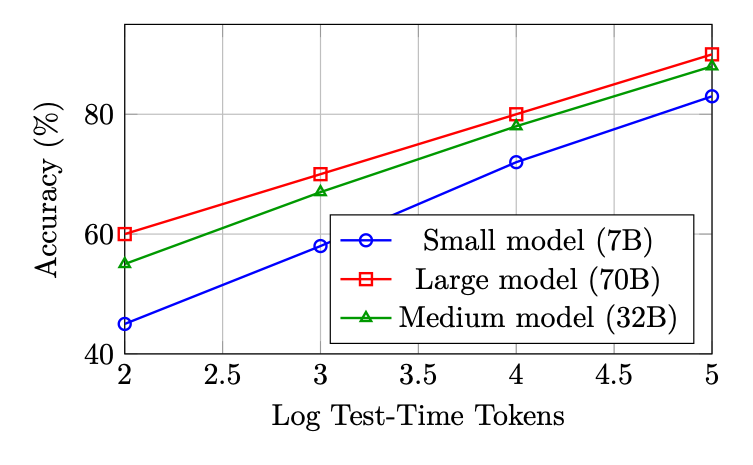
\includegraphics[width=0.85\textwidth]{figures/fig_044_test_time_scaling.png}
% \caption{Schematic test-time compute scaling curves. Performance improves log-linearly with inference tokens across model sizes, and smaller models with more compute can approach larger models with less compute.}
\caption{测试时算力扩展曲线示意图。在各种模型规模下，性能随推理 Token 数对数线性提升；较小模型在更多算力下可以逼近较大模型在更少算力下的表现。}
\label{fig:test_time_scaling}
\end{figure}

% The practical implication is profound: \textbf{reasoning models trade training compute for inference compute}. Rather than always deploying the largest possible model, one can deploy a smaller, reasoning-capable model and allocate more tokens to ``thinking'' on hard problems.
其实践含义深远：\textbf{推理模型用推理算力换取训练算力}。不必总是部署尽可能大的模型，而是可以部署一个具备推理能力的较小模型，并在难题上分配更多 Token 用于“思考”。

\section{测试时扩展方法}
\label{sec:test_time_methods}

% The scaling laws above show that investing more compute at inference can dramatically improve reasoning performance. This section provides a comprehensive treatment of the \textbf{methods} that operationalize test-time scaling --- from simple chain-of-thought to sophisticated tree and graph search algorithms. These methods form a spectrum trading inference cost for accuracy, and understanding their structure is essential for designing modern reasoning systems.
上述扩展律表明，在推理阶段投入更多算力可以显著提升推理性能。本节系统介绍将测试时扩展（Test-Time Scaling）落地的各类\textbf{方法}——从简单的思维链到复杂的树与图搜索算法。这些方法构成了一个用推理成本换取准确率的连续谱，理解其结构对于设计现代推理系统至关重要。

\begin{figure}[ht!]
\centering
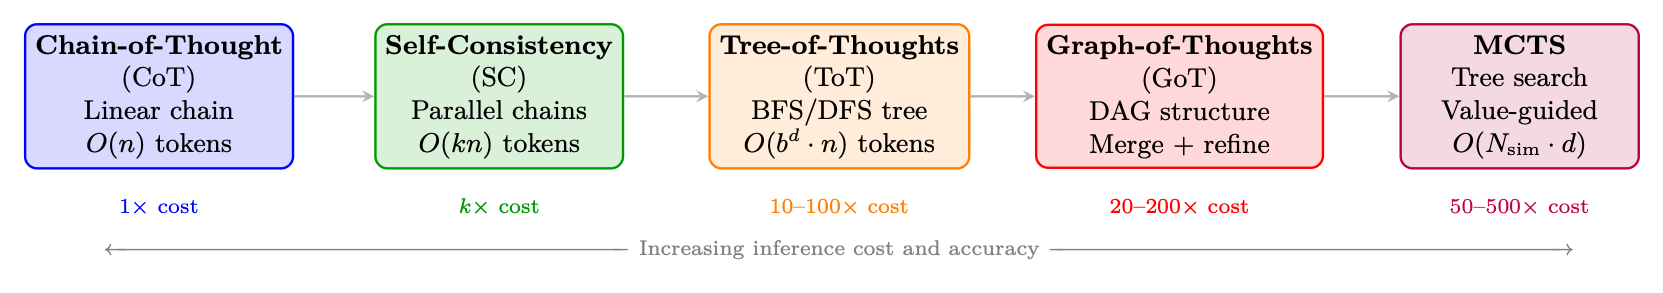
\includegraphics[width=\textwidth]{figures/fig_045_test_time_spectrum.png}
% \caption{Spectrum of test-time scaling methods. Each method trades additional inference compute for improved reasoning accuracy. Methods build on each other conceptually: CoT introduces explicit reasoning, Self-Consistency adds sampling, ToT adds structured search, GoT adds merging operations, and MCTS adds learned value guidance.}
\caption{测试时扩展方法的连续谱。每种方法都以额外的推理算力换取更高的推理准确率。各方法在概念上层层递进：CoT 引入显式推理，Self-Consistency 加入采样，ToT 引入结构化搜索，GoT 加入合并操作，而 MCTS 加入学习到的价值引导。}
\label{fig:test_time_spectrum}
\end{figure}

\subsection{思维链（CoT）}
\label{subsec:cot_method}

% Chain-of-Thought prompting~\cite{wei2022chain} is the foundation of all test-time scaling methods. Rather than directly outputting an answer, the model generates intermediate reasoning steps that decompose complex problems into manageable sub-problems.
思维链 Prompt~\cite{wei2022chain} 是所有测试时扩展方法的基础。模型不再直接输出答案，而是生成中间推理步骤，将复杂问题分解为可处理的子问题。

\paragraph{零样本 CoT。}
\label{zero-shot-cot.}

% Kojima et al.~\cite{kojima2022large} demonstrated that appending ``Let’s think step by step'' to a prompt elicits reasoning behavior without any exemplars. This simple trigger activates latent reasoning capabilities in sufficiently large models ($\geq$100B parameters).
Kojima 等~\cite{kojima2022large} 证明，仅在 Prompt 末尾追加“Let's think step by step”就能在没有任何示例的情况下激发推理行为。这一简单触发器可以激活足够大模型（$\geq$ 100B 参数）中的潜在推理能力。

\paragraph{少样本 CoT。}
\label{few-shot-cot.}

% Wei et al.~\cite{wei2022chain} showed that providing a few exemplars with explicit reasoning traces enables smaller models to reason effectively:
Wei 等~\cite{wei2022chain} 表明，提供少量带有显式推理轨迹的示例能够让较小的模型也有效地进行推理：
\begin{equation}
\text{Prompt} = [(x_1, z_1, y_1), (x_2, z_2, y_2), \ldots, (x_k, z_k, y_k), (x_{\text{test}}, \texttt{?})]
\end{equation}
% where $z_i$ are hand-written reasoning traces for exemplar $(x_i, y_i)$.
其中 $z_i$ 是为示例 $(x_i, y_i)$ 手工编写的推理轨迹。

\paragraph{形式化刻画。}
\label{formal-characterization.}

% CoT converts a single-step prediction $p(y|x)$ into a multi-step sequential generation:
CoT 将单步预测 $p(y|x)$ 转化为多步序列生成：
\begin{equation}
p(y|x) = \sum_{z} p(y|x, z) \cdot p(z|x) \approx p(y|x, z^*) \cdot p(z^*|x)
\end{equation}
% where $z^* = (z_1, z_2, \ldots, z_T)$ is the greedy reasoning chain. The summation over all possible chains is intractable; standard CoT uses a single sample (greedy or temperature sampling).
其中 $z^* = (z_1, z_2, \ldots, z_T)$ 是贪心推理链。对所有可能链条求和是不可计算的；标准 CoT 仅采用单一样本（贪心或温度采样）。

\paragraph{局限性。}
\label{limitations.-dup2}

% Single-chain CoT is fragile: if an early reasoning step is wrong, all subsequent steps build on a flawed foundation with no mechanism for recovery.
单链 CoT 是脆弱的：一旦早期推理步骤出错，后续所有步骤都会建立在错误基础上，且没有任何恢复机制。

\subsection{自洽性（多数投票）}
\label{self-consistency-majority-voting}

% Self-Consistency~\cite{wang2023selfconsistency} addresses CoT’s single-chain fragility by sampling \textbf{multiple independent reasoning chains} and taking a majority vote over the final answers:
自洽性（Self-Consistency）~\cite{wang2023selfconsistency} 通过采样\textbf{多条独立的推理链}并对最终答案取多数投票，来缓解 CoT 单链脆弱的问题：
\begin{equation}
\hat{y} = \arg\max_{y} \sum_{i=1}^{N} \mathbf{1}[y_i = y], \quad \text{where } (z_i, y_i) \sim p(\cdot | x), \; T > 0
\end{equation}

\textbf{关键性质}：

\begin{itemize}
  % \item Uses temperature $T > 0$ sampling to generate diverse chains (typically $T = 0.7$--$1.0$)
  \item 使用温度 $T > 0$ 的采样以产生多样的链条（通常 $T = 0.7$--$1.0$）
  % \item No interaction between chains --- fully parallelizable
  \item 链条之间无交互——完全可并行化
  % \item Accuracy improves monotonically with $N$ (diminishing returns after $N \approx 40$)
  \item 准确率随 $N$ 单调提升（$N \approx 40$ 之后收益递减）
  % \item On GSM8K: CoT = 56.5\%, Self-Consistency ($N$=40) = 74.4\% (with PaLM-540B~\cite{chowdhery2022palm})
  \item 在 GSM8K 上：CoT = 56.5\%，Self-Consistency（$N$=40）= 74.4\%（使用 PaLM-540B~\cite{chowdhery2022palm}）
  % \item Equivalent to \textbf{Best-of-N with outcome reward} (majority vote acts as implicit ORM)
  \item 等价于\textbf{使用结果奖励的 Best-of-N}（多数投票充当隐式的 ORM）
\end{itemize}

\begin{intuitionbox}[多数投票为何有效]
% If the model has probability $p > 0.5$ of generating a correct reasoning chain, then by the law of large numbers, majority voting over $N$ independent samples approaches 100\% accuracy as $N \to \infty$. Even with $p = 0.3$ (model is usually wrong), if correct answers concentrate on one value while incorrect answers are diverse, majority voting still recovers the correct answer. This is the statistical foundation of test-time scaling.
若模型生成正确推理链的概率为 $p > 0.5$，则由大数定律可知：当 $N \to \infty$ 时，对 $N$ 个独立样本做多数投票的准确率趋近 100\%。即便 $p = 0.3$（模型通常是错的），只要正确答案集中在某一个值上、而错误答案彼此分散，多数投票仍能恢复出正确答案。这是测试时扩展的统计基础。
\end{intuitionbox}

\subsection{思维树（ToT）}
\label{subsec:tot_method}

% Tree-of-Thoughts~\cite{yao2024tree} generalizes CoT from a \textbf{linear chain} to a \textbf{tree structure}, enabling the model to explore multiple reasoning paths, evaluate intermediate states, and backtrack from unpromising branches. This introduces deliberate planning into the reasoning process.
思维树（Tree-of-Thoughts，ToT）~\cite{yao2024tree} 将 CoT 从\textbf{线性链}推广为\textbf{树形结构}，使模型能够探索多条推理路径、评估中间状态，并从前景不佳的分支回溯。这为推理过程引入了刻意的规划。

\paragraph{核心抽象。}
\label{core-abstraction.}

% A reasoning problem is decomposed into a search over a tree where:
推理问题被分解为对一棵树的搜索，其中：

\begin{itemize}
  % \item \textbf{Root}: Initial problem statement $x$
  \item \textbf{根节点}：初始问题陈述 $x$
  % \item \textbf{Nodes}: Partial reasoning states $s = (x, z_1, \ldots, z_k)$
  \item \textbf{节点}：部分推理状态 $s = (x, z_1, \ldots, z_k)$
  % \item \textbf{Edges}: Individual reasoning steps (``thoughts'') $z_{k+1}$
  \item \textbf{边}：单个推理步骤（“想法”）$z_{k+1}$
  % \item \textbf{Leaves}: Complete solutions with final answers
  \item \textbf{叶子}：包含最终答案的完整解答
  % \item \textbf{Value function}: $V(s)$ estimates how promising a partial solution is
  \item \textbf{价值函数}：$V(s)$ 估计某个部分解的前景如何
\end{itemize}

\paragraph{形式化定义。}
\label{formal-definition.}

\begin{equation}
\text{ToT} = (\mathcal{G}, \mathcal{E}, V, \pi_\theta, \text{Search})
\end{equation}
其中：

\begin{itemize}
  % \item $\mathcal{G}$: \textbf{Thought generator} --- produces $b$ candidate next thoughts: $\{z^{(1)}, \ldots, z^{(b)}\} \sim \pi_\theta(\cdot | s)$
  \item $\mathcal{G}$：\textbf{想法生成器}——产生 $b$ 个候选的下一想法：$\{z^{(1)}, \ldots, z^{(b)}\} \sim \pi_\theta(\cdot | s)$
  % \item $\mathcal{E}$: \textbf{State evaluator} --- scores partial solutions: $V(s) \in \{$\emph{sure}, \emph{maybe}, \emph{impossible}$\}$ or $V(s) \in [0, 1]$
  \item $\mathcal{E}$：\textbf{状态评估器}——为部分解打分：$V(s) \in \{$\emph{sure}, \emph{maybe}, \emph{impossible}$\}$ 或 $V(s) \in [0, 1]$
  % \item $\pi_\theta$: The language model generating thoughts
  \item $\pi_\theta$：生成想法的语言模型
  % \item $\text{Search}$: Search algorithm (BFS or DFS)
  \item $\text{Search}$：搜索算法（BFS 或 DFS）
\end{itemize}

\begin{figure}[ht!]
\centering
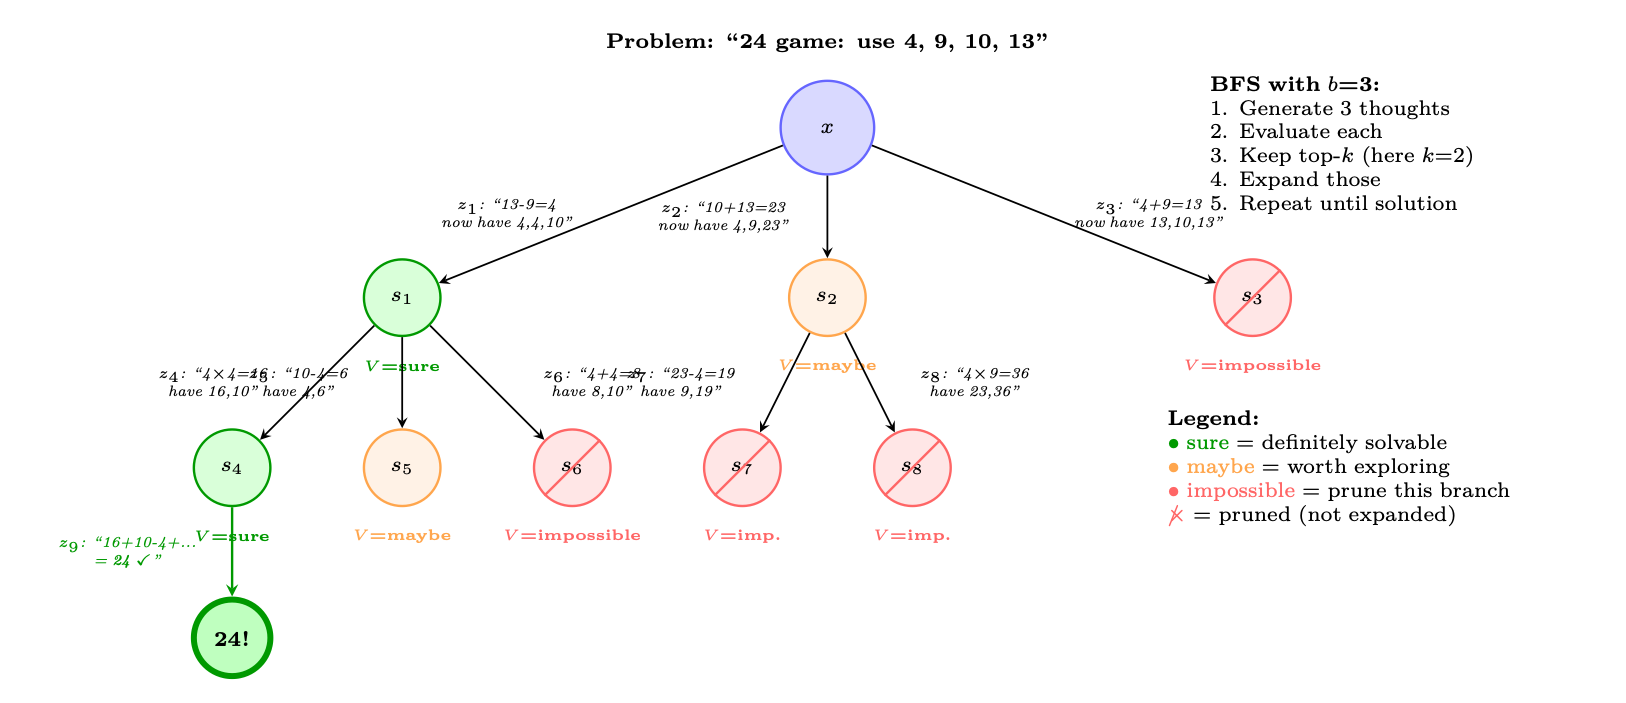
\includegraphics[width=0.85\textwidth]{figures/fig_046_tot_example.png}
% \caption{Tree-of-Thoughts on the ``Game of 24'' task: use operations on {4, 9, 10, 13} to make 24. At each level, the model generates $b=3$ candidate thoughts, evaluates each (sure/maybe/impossible), prunes unpromising branches, and expands the most promising ones. The green path leads to a solution; red paths are pruned early.}
\caption{思维树在“24 点”任务上的运行：对 {4, 9, 10, 13} 进行四则运算得到 24。在每一层，模型生成 $b=3$ 个候选想法，分别评估（sure/maybe/impossible），剪掉前景不佳的分支，并扩展最有希望的分支。绿色路径通向解答；红色路径在早期被剪枝。}
\end{figure}

\paragraph{搜索算法。}
\label{search-algorithms.}

\textbf{BFS（广度优先搜索）：}

\begin{enumerate}
  % \item Generate $b$ candidate thoughts for each node at current depth
  \item 为当前深度的每个节点生成 $b$ 个候选想法
  % \item Evaluate all candidates with $V(\cdot)$
  \item 用 $V(\cdot)$ 评估所有候选
  % \item Keep top-$k$ most promising states (beam search)
  \item 保留前 $k$ 个最有希望的状态（束搜索）
  % \item Advance all $k$ states to the next level
  \item 将这 $k$ 个状态全部推进到下一层
  % \item Repeat until a solution is found or depth limit reached
  \item 重复，直到找到解答或达到深度上限
\end{enumerate}

\textbf{DFS（深度优先搜索）：}

\begin{enumerate}
  % \item Generate $b$ candidate thoughts for current state
  \item 为当前状态生成 $b$ 个候选想法
  % \item Evaluate: if $V(s) =$ \emph{impossible}, backtrack immediately
  \item 评估：若 $V(s) =$ \emph{impossible}，立即回溯
  % \item If $V(s) =$ \emph{sure/maybe}, recurse deeper (pick the most promising)
  \item 若 $V(s) =$ \emph{sure/maybe}，向更深处递归（选择最有希望的一个）
  % \item If depth limit reached without solution, backtrack
  \item 若达到深度上限仍未得到解答，则回溯
  % \item Continue until solution found or all branches explored
  \item 继续直到找到解答或所有分支都被探索完
\end{enumerate}

\begin{examplebox}[ToT：价值评估 Prompt]
\begin{lstlisting}[style=pythonstyle]
# LLM 用于评估部分推理状态：
EVAL_PROMPT = """Evaluate if this partial solution can reach 24.

Numbers remaining: [4, 4, 10]
Steps so far: 13 - 9 = 4

Can these remaining numbers (4, 4, 10) be combined using +,-,*,/
to make 24?

Analysis: 4 * (10 - 4) = 4 * 6 = 24. Yes!

Judge: sure/maybe/impossible
Answer: sure"""

# 想法生成 Prompt：
GEN_PROMPT = """Input: 4 9 10 13
Possible next steps:
1. 13 - 9 = 4 (left: 4 4 10)
2. 10 + 13 = 23 (left: 4 9 23)
3. 9 - 4 = 5 (left: 5 10 13)
..."""
\end{lstlisting}
\end{examplebox}

\paragraph{计算成本。}
\label{computational-cost.}

% For ToT with branching factor $b$, depth $d$, and beam width $k$:
对于分支因子为 $b$、深度为 $d$、束宽为 $k$ 的 ToT：
\begin{equation}
\text{LLM calls (BFS)} = \underbrace{k \cdot b}_{\text{generation}} + \underbrace{k \cdot b}_{\text{evaluation}} = 2kb \text{ per level} \implies \text{Total} = 2kbd
\end{equation}
% For the 24 game: $b=3, k=2, d=3 \implies 36$ LLM calls vs.~1 for standard CoT.
对于 24 点游戏：$b=3, k=2, d=3 \implies 36$ 次 LLM 调用，而标准 CoT 仅需 1 次。

\paragraph{结果。}
\label{results.-dup2}

% On the Game of 24 (a challenging arithmetic reasoning task), ToT achieves 74\% success rate vs.~CoT’s 4\% --- a massive improvement from structured search over the same base model (GPT-4).
在 24 点游戏（一个具挑战性的算术推理任务）上，ToT 达到 74\% 的成功率，而 CoT 仅 4\%——在相同基础模型（GPT-4）之上，结构化搜索带来了巨大的提升。

\subsection{思维图（GoT）}
\label{subsec:got_method}

% Graph-of-Thoughts~\cite{besta2024graph} extends ToT from a tree to a \textbf{directed acyclic graph (DAG)}, introducing a critical capability: \textbf{merging} partial solutions from different branches. This allows the model to synthesize insights from multiple reasoning paths into a single refined solution.
思维图（Graph-of-Thoughts，GoT）~\cite{besta2024graph} 将 ToT 从树推广到\textbf{有向无环图（DAG）}，引入了一项关键能力：\textbf{合并}来自不同分支的部分解。这让模型可以把多条推理路径中的洞见综合到一个精炼的解答中。

\paragraph{关键操作。}
\label{key-operations.}

% GoT introduces three operations beyond ToT:
GoT 在 ToT 之上引入了三种操作：

\begin{itemize}
  % \item \textbf{Generate}: Produce new thoughts from a state (same as ToT)
  \item \textbf{Generate}：从一个状态产生新的想法（与 ToT 相同）
  % \item \textbf{Aggregate/Merge}: Combine multiple thoughts into one refined thought --- this is impossible in a tree
  \item \textbf{Aggregate/Merge}：把多个想法合并为一个更精炼的想法——这是树结构中不可能做到的
  % \item \textbf{Refine}: Iteratively improve a thought based on feedback
  \item \textbf{Refine}：基于反馈对一个想法进行迭代改进
  % \item \textbf{Score}: Evaluate thought quality (same as ToT’s value function)
  \item \textbf{Score}：评估想法的质量（与 ToT 的价值函数相同）
\end{itemize}

\begin{figure}[ht!]
\centering
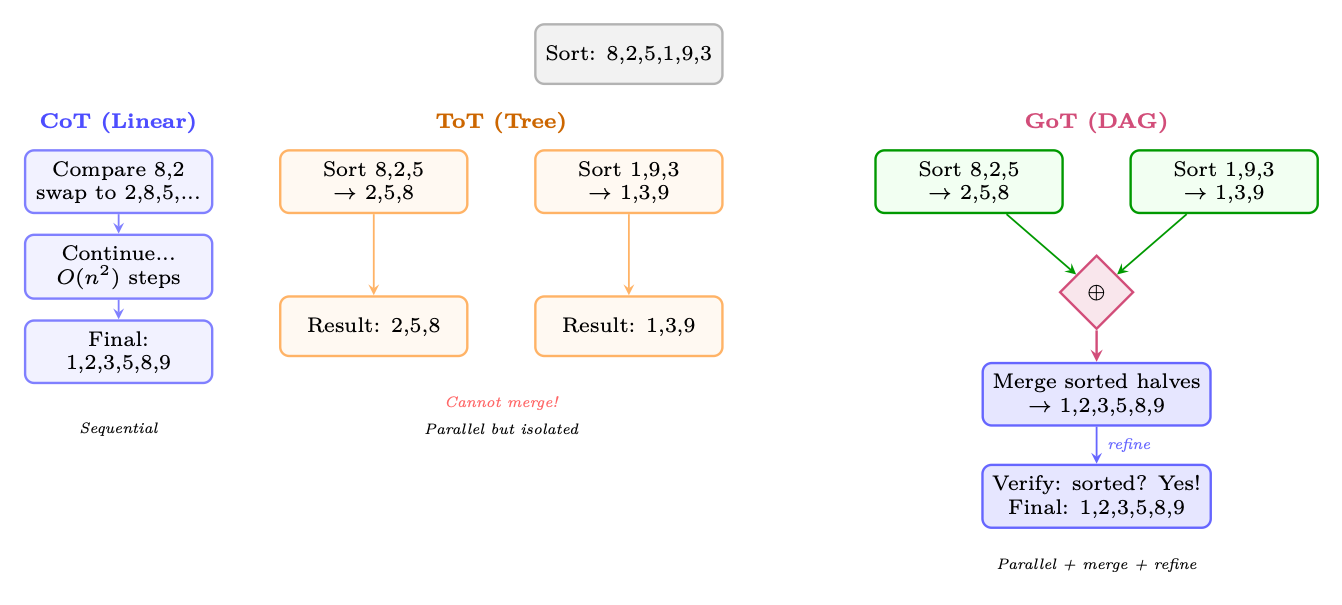
\includegraphics[width=0.85\textwidth]{figures/fig_047_got_comparison.png}
% \caption{Comparison of CoT (linear chain), ToT (tree --- branches but no merging), and GoT (DAG --- branches can merge). For a sorting task, GoT can split the array into sub-problems, solve them independently (parallel), then \textbf{merge} the results --- impossible in a pure tree structure. This enables divide-and-conquer reasoning.}
\caption{CoT（线性链）、ToT（树——只能分支不能合并）与 GoT（DAG——分支可以合并）的对比。对于一个排序任务，GoT 可以把数组拆为子问题、独立（并行）求解，然后\textbf{合并}结果——在纯树结构中不可能做到。这使得分治式推理成为可能。}
\label{fig:got_comparison}
\end{figure}

\paragraph{图操作（形式化）。}
\label{graph-operations-formal.}

% Let $\mathcal{V} = \{v_1, \ldots, v_n\}$ be thought vertices and $\mathcal{E} \subseteq \mathcal{V} \times \mathcal{V}$ be directed edges. GoT supports:
设 $\mathcal{V} = \{v_1, \ldots, v_n\}$ 为想法节点，$\mathcal{E} \subseteq \mathcal{V} \times \mathcal{V}$ 为有向边。GoT 支持：
\begin{align}
\textbf{Generate}(v) &: v \to \{v_{c_1}, \ldots, v_{c_b}\} && \text{(创建子节点)} \\
\textbf{Aggregate}(v_1, \ldots, v_k) &\to v_{\text{merged}} && \text{(将 $k$ 个想法合并为一个)} \\
\textbf{Refine}(v, n) &\to v' && \text{(通过 $n$ 次迭代改进 $v$)} \\
\textbf{Score}(v) &\to s \in [0, 1] && \text{(评估想法质量)}
\end{align}

% The \textbf{Aggregate} operation is the key differentiator: it creates edges from multiple parent nodes to a single child, forming a DAG rather than a tree. This enables:
\textbf{Aggregate} 操作是关键差异：它从多个父节点向单个子节点连边，从而形成 DAG 而非树。这使得以下能力成为可能：

\begin{itemize}
  % \item \textbf{Divide-and-conquer}: Split problem $\to$ solve sub-problems in parallel $\to$ merge solutions
  \item \textbf{分治}：拆分问题 $\to$ 并行求解子问题 $\to$ 合并解答
  % \item \textbf{Ensemble reasoning}: Generate multiple perspectives, then synthesize the best ideas
  \item \textbf{集成推理}：生成多个视角，然后综合出最佳想法
  % \item \textbf{Iterative refinement}: Feed evaluation results back to improve earlier thoughts
  \item \textbf{迭代精炼}：把评估结果反馈回去以改进早期想法
\end{itemize}

\paragraph{结果。}
\label{results.-1}

% On sorting (a task requiring merging), GoT achieves 62\% cost reduction vs.~ToT at equivalent quality. On set intersection and keyword counting, GoT matches ToT quality with 30--40\% fewer LLM calls due to the merge operation enabling more efficient decomposition.
在排序任务（一项需要合并的任务）上，GoT 在质量相当时相比 ToT 节省 62\% 成本。在集合求交与关键词计数任务上，由于合并操作支持更高效的分解，GoT 在相同质量下减少了 30--40\% 的 LLM 调用。

\subsection{结合奖励模型的 Best-of-N}
\label{subsec:bon_method}

% Best-of-N (BoN)~\cite{nakano2021webgpt, stiennon2020learning} is the simplest scaling method that uses a \textbf{learned reward model} to select among candidates:
Best-of-N 采样（Rejection Sampling）（BoN）~\cite{nakano2021webgpt, stiennon2020learning} 是最简单的扩展方法，它利用一个\textbf{学习得到的奖励模型}在候选中进行选择：
\begin{equation}
y^* = \arg\max_{y \in \{y_1, \ldots, y_N\}} R_\phi(x, y), \quad y_i \sim \pi_\theta(\cdot | x)
\end{equation}

\textbf{按奖励模型类型的变体}：

\begin{itemize}
  % \item \textbf{BoN with ORM}: Score complete solutions; select the highest-scoring one. Equivalent to Self-Consistency when ORM $\approx$ correctness check.
  \item \textbf{结合 ORM 的 BoN}：对完整解答打分，选择得分最高者。当 ORM $\approx$ 正确性检查时等价于 Self-Consistency。
  % \item \textbf{BoN with PRM}: Score at each reasoning step; select the solution with highest minimum step score (least likely to have an error at any step).
  \item \textbf{结合 PRM 的 BoN}：对每一推理步打分，选择最小步得分最高的解答（即在任何步骤上出错的可能性最小）。
  % \item \textbf{Weighted BoN}: Weight candidates by reward: $y^* \sim \text{softmax}(R(y_1)/\tau, \ldots, R(y_N)/\tau)$.
  \item \textbf{加权 BoN}：按奖励对候选加权：$y^* \sim \text{softmax}(R(y_1)/\tau, \ldots, R(y_N)/\tau)$。
\end{itemize}

\begin{keybox}[BoN 扩展律]
% For a model with per-sample accuracy $p$, the probability of at least one correct sample in $N$ tries:
对于单样本准确率为 $p$ 的模型，$N$ 次采样中至少有一个正确样本的概率为：
\begin{equation}
P(\text{success with BoN}) = 1 - (1-p)^N
\end{equation}
% With a perfect reward model (oracle that always selects correctly):
在完美奖励模型（总能正确选择的预言机）下：

\begin{itemize}
  \item $p = 0.3, N = 10$：成功率 = $97\%$
  \item $p = 0.1, N = 50$：成功率 = $99.5\%$
\end{itemize}

% In practice, imperfect reward models cap the effective $N$ --- beyond $N \approx 64$--$256$, reward model errors dominate and accuracy plateaus or decreases (\textbf{reward hacking}).
在实践中，不完美的奖励模型会限制有效的 $N$——超过 $N \approx 64$--$256$ 后，奖励模型的误差开始主导，准确率趋于停滞甚至下降（\textbf{奖励黑客}）。
\end{keybox}

\subsection{面向推理的蒙特卡洛树搜索（MCTS）}
\label{monte-carlo-tree-search-mcts-for-reasoning}

% MCTS~\cite{kocsis2006bandit, silver2016mastering} combines the structured exploration of ToT with \textbf{learned value estimates} and \textbf{visit-count statistics} to allocate inference compute optimally. Originally developed for game-playing (AlphaGo~\cite{silver2016mastering}), MCTS has been adapted for LLM reasoning by systems including AlphaProof~\cite{alphaproof2024} and rStar~\cite{qi2024mutual}.
蒙特卡洛树搜索（MCTS）~\cite{kocsis2006bandit, silver2016mastering} 将 ToT 的结构化探索与\textbf{学习到的价值估计}及\textbf{访问计数统计}结合起来，从而最优地分配推理算力。MCTS 最初为博弈而设计（AlphaGo~\cite{silver2016mastering}），后被 AlphaProof~\cite{alphaproof2024}、rStar~\cite{qi2024mutual} 等系统改造用于 LLM 推理。

\paragraph{算法（针对 LLM 推理改造）。}
\label{algorithm-adapted-for-llm-reasoning.}

% Each MCTS iteration consists of four phases:
每次 MCTS 迭代包含四个阶段：

\begin{figure}[ht!]
\centering
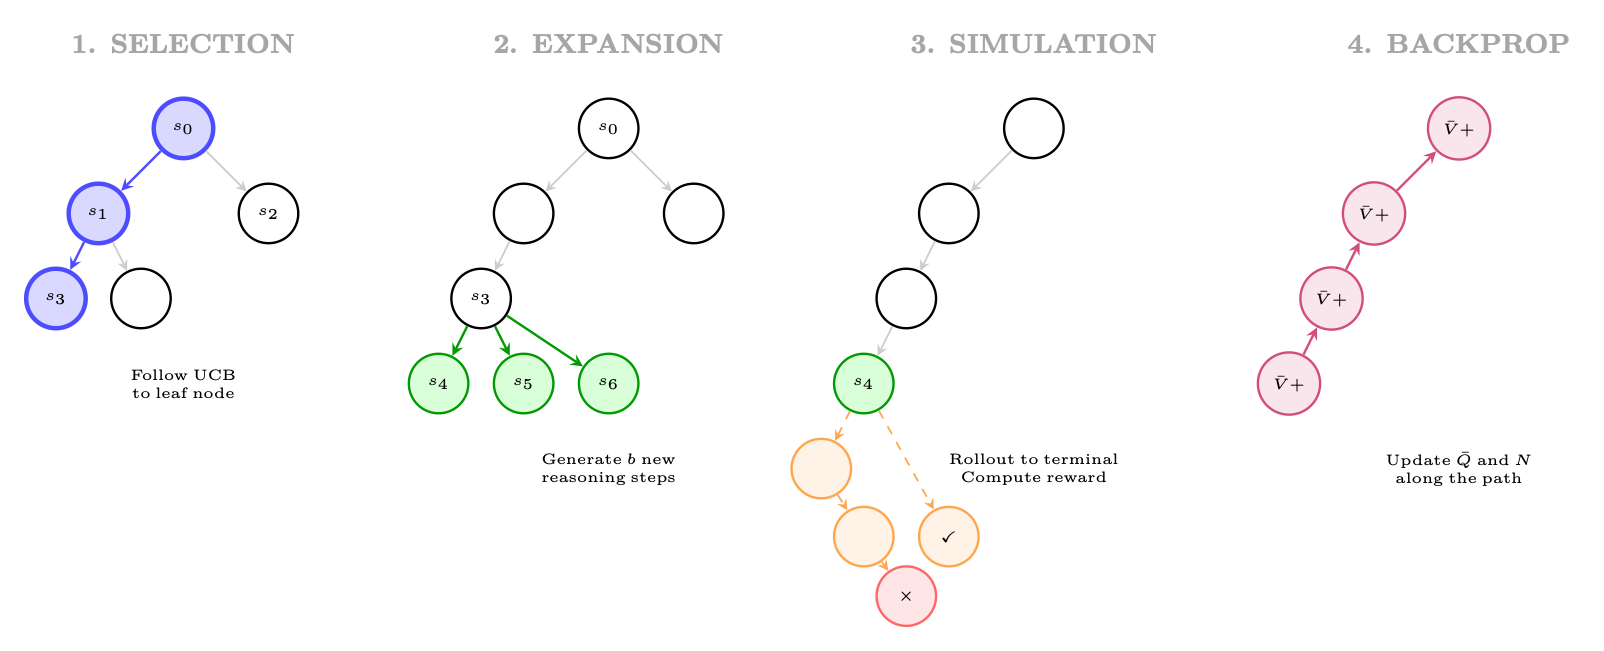
\includegraphics[width=0.85\textwidth]{figures/fig_048_mcts_phases.png}
% \caption{Four phases of MCTS for reasoning: (1) \textbf{Selection}: traverse tree using UCB to find a promising leaf; (2) \textbf{Expansion}: generate new reasoning steps from the leaf; (3) \textbf{Simulation}: complete the reasoning to a terminal state and evaluate; (4) \textbf{Backpropagation}: update value estimates along the path.}
\caption{面向推理的 MCTS 的四个阶段：(1) \textbf{选择}：用 UCB 遍历树以找到一个有前途的叶子节点；(2) \textbf{扩展}：从该叶子节点生成新的推理步骤；(3) \textbf{模拟}：将推理补全到终止状态并进行评估；(4) \textbf{反向传播}：沿路径更新价值估计。}
\label{fig:mcts_phases}
\end{figure}

\paragraph{推理中的 UCB。}
\label{ucb-for-reasoning.}

% Node selection uses PUCT (Predictor + UCB applied to Trees):
节点选择使用 PUCT（Predictor + UCB applied to Trees）：
\begin{equation}
a^* = \arg\max_a \left[ Q(s, a) + c_{\text{puct}} \cdot P(s, a) \cdot \frac{\sqrt{\sum_b N(s,b)}}{1 + N(s, a)} \right]
\end{equation}
% where $P(s,a) = \pi_\theta(a|s)$ is the LLM’s prior probability of generating step $a$ from state $s$. This biases exploration toward steps the LLM already considers likely, while the UCB term encourages trying under-explored alternatives.
其中 $P(s,a) = \pi_\theta(a|s)$ 是 LLM 从状态 $s$ 生成步骤 $a$ 的先验概率。这使探索偏向 LLM 本就认为可能的步骤，而 UCB 项鼓励尝试探索不足的备选方案。

\begin{examplebox}[面向数学推理的 MCTS：运行示例]
\textbf{问题}：证明 $\sqrt{2}$ 是无理数。

\textbf{第 1 次迭代}（Selection $\to$ 根节点，Expansion）：

\begin{itemize}
  % \item Generate 3 candidate first steps:
  \item 生成 3 个候选的首步：

\begin{enumerate}
  \item “Assume for contradiction that $\sqrt{2} = p/q$ in lowest terms.”（$P = 0.7$）
  \item “Consider the decimal expansion of $\sqrt{2}$ = 1.414...”（$P = 0.15$）
  \item “Use the fundamental theorem of arithmetic.”（$P = 0.10$）
\end{enumerate}
  % \item Rollout from $z_1$: reaches correct proof in 4 steps $\to$ $r = 1.0$
  \item 从 $z_1$ 做 Rollout：4 步内得到正确证明 $\to$ $r = 1.0$
  % \item Rollout from $z_2$: fails (decimal doesn’t prove irrationality) $\to$ $r = 0.0$
  \item 从 $z_2$ 做 Rollout：失败（小数展开不能证明无理性）$\to$ $r = 0.0$
  % \item Backprop: $Q(s_0, z_1) = 1.0$, $N(s_0, z_1) = 1$
  \item 反向传播：$Q(s_0, z_1) = 1.0$，$N(s_0, z_1) = 1$
\end{itemize}

\textbf{第 2 次迭代}（Selection：按 UCB 选中 $z_1$）：

\begin{itemize}
  % \item Expand from state ``Assume $\sqrt{2} = p/q$...'':
  \item 从状态“Assume $\sqrt{2} = p/q$...”进行扩展：

\begin{enumerate}
  \item “Then $2 = p^2/q^2$, so $p^2 = 2q^2$.”（$P = 0.8$）
  \item “Then $p$ and $q$ share no common factors.”（$P = 0.15$）
\end{enumerate}
  % \item Rollout from $z_4$: correct continuation $\to r = 1.0$
  \item 从 $z_4$ 做 Rollout：正确续推 $\to r = 1.0$
  % \item Backprop: $Q(s_0, z_1) = 1.0$, $Q(s_1, z_4) = 1.0$
  \item 反向传播：$Q(s_0, z_1) = 1.0$，$Q(s_1, z_4) = 1.0$
\end{itemize}

% \textbf{After 20 iterations}: The tree has explored 8 distinct reasoning paths. The most-visited path is selected as the final proof: $z_1 \to z_4 \to z_6 \to z_8$ (classical proof by contradiction via even/odd argument).
\textbf{20 次迭代之后}：树已探索 8 条不同的推理路径。访问次数最多的路径被选为最终证明：$z_1 \to z_4 \to z_6 \to z_8$（基于奇偶性论证的经典反证法）。
\end{examplebox}

\paragraph{对比：ToT vs.~MCTS。}
\label{comparison-tot-vs.-mcts.}

\begin{table}[ht!]
\centering\small
% \caption{Tree-of-Thoughts vs.~Monte Carlo Tree Search for reasoning.}
\caption{面向推理的 Tree-of-Thoughts 与 Monte Carlo Tree Search 对比。}
\noindent\begin{tabularx}{\linewidth}{@{}l Z{0.92} Z{1.08}@{}}
\toprule
\textbf{维度} & \textbf{ToT} & \textbf{MCTS} \\
\midrule
价值估计 & LLM Prompt（“sure/maybe/impossible”） & 学习得到的价值网络 + Rollout 统计 \\
探索方式 & 固定束宽；不回访 & UCB 自适应地把预算分配给有前途的节点 \\
算力分配 & 各深度层均匀 & 聚焦：在更难的子问题上做更多模拟 \\
训练集成 & 无训练；纯 Prompt & 可将 MCTS 策略蒸馏回基础模型~\cite{silver2016mastering} \\
最适用于 & 分支简单的问题（24 点） & 需要深度探索的复杂问题（证明、代码） \\
\bottomrule
\end{tabularx}
\end{table}

\subsection{推理步级的束搜索}
\label{subsec:beam_reasoning}

% Beam search --- long standard in NMT and text generation --- can be applied at the \emph{reasoning step} level rather than the token level. Instead of tracking the top-$k$ token sequences, we track the top-$k$ \textbf{reasoning prefixes}:
束搜索——在 NMT 与文本生成中长期作为标准方法——也可以在\emph{推理步}层面而非 Token 层面应用。我们不再跟踪前 $k$ 个 Token 序列，而是跟踪前 $k$ 个\textbf{推理前缀}：

\begin{equation}
\mathcal{B}_d = \text{top-}k\left\{ (s_1, \ldots, s_d) : \sum_{i=1}^d \log \pi_\theta(s_i | s_{<i}) + \lambda \cdot V_\phi(s_1, \ldots, s_d) \right\}
\end{equation}

% where the scoring combines the LLM log-probability (fluency) with a value model estimate (correctness). This is effectively ToT-BFS with a learned value function rather than a prompted one.
其中评分将 LLM 的对数概率（流畅性）与价值模型估计（正确性）相结合。这本质上是用学习到的价值函数取代提示式价值函数的 ToT-BFS。

\subsection{迭代精炼与自我纠正}
\label{iterative-refinement-and-self-correction}

% Rather than exploring \emph{breadth} (multiple parallel chains), iterative refinement invests compute in \emph{depth} --- repeatedly improving a single solution:
与探索\emph{广度}（多条并行链）不同，迭代精炼把算力投入到\emph{深度}——反复改进同一个解答：

\begin{equation}
y^{(t+1)} = \text{LLM}\!\left(\text{``Improve this solution:''}, y^{(t)}, \text{``Errors found:''}, e^{(t)}\right)
\end{equation}

其中 $e^{(t)}$ 可来自：

\begin{itemize}
  % \item \textbf{Self-verification}: Ask the model to check its own answer
  \item \textbf{自我验证}：让模型检查自己的答案
  % \item \textbf{External verification}: Run code, check math symbolically
  \item \textbf{外部验证}：运行代码、符号化地校验数学
  % \item \textbf{Critic model}: A separate model identifies errors
  \item \textbf{评判模型}：由一个独立模型识别错误
\end{itemize}

% Notable methods: \textbf{Self-Refine}~\cite{madaan2023selfrefine} (iterative self-feedback), \textbf{Reflexion}~\cite{shinn2023reflexion} (verbal RL via reflections stored in memory), and \textbf{LATS}~\cite{zhou2024lats} (tree search + reflection-based pruning).
代表性方法：\textbf{Self-Refine}~\cite{madaan2023selfrefine}（迭代自我反馈）、\textbf{Reflexion}~\cite{shinn2023reflexion}（通过存入记忆的反思实现的语言化 RL）以及 \textbf{LATS}~\cite{zhou2024lats}（树搜索 + 基于反思的剪枝）。

\subsection{方法对比与选型指南}
\label{method-comparison-and-selection-guide}

\begin{table}[ht!]
\centering
% \caption{Comprehensive comparison of test-time scaling methods.}
\caption{测试时扩展方法的综合比较。}
{\footnotesize
\noindent\begin{tabularx}{\linewidth}{@{}Z{1.05} l l l l Z{0.95}@{}}
\toprule
\textbf{方法} & \textbf{结构} & \textbf{LLM 调用} & \textbf{可并行} & \textbf{需要 RM？} & \textbf{最适用于} \\
\midrule
CoT~\cite{wei2022chain} & 链 & 1 & N/A & 否 & 简单—中等难度问题 \\
Self-Consistency~\cite{wang2023selfconsistency} & 并行链 & $N$ & \checkmark{} 完全 & 否（多数投票） & 答案离散的数学题 \\
Best-of-N + ORM & 并行链 & $N$ + 1 & \checkmark{} 完全 & 是（ORM） & 有良好 RM 的通用任务 \\
Best-of-N + PRM & 并行链 & $N$ + $N{\cdot}K$ & \checkmark{} 完全 & 是（PRM） & 复杂多步推理 \\
ToT~\cite{yao2024tree} & 树（BFS/DFS） & $O(kbd)$ & 部分 & LLM 作判官 & 结构化搜索问题 \\
GoT~\cite{besta2024graph} & DAG & $O(kbd)$ & 部分 & LLM 作判官 & 可分解的问题 \\
MCTS~\cite{kocsis2006bandit} & 树 + 价值 & $O(N_{\text{sim}} \cdot d)$ & 部分 & 是（价值网络） & 困难证明、编程 \\
Self-Refine~\cite{madaan2023selfrefine} & 线性（迭代） & $2T$ & 否 & 自我评判 & 开放式生成 \\
LATS~\cite{zhou2024lats} & 树 + 反思 & $O(N \cdot d)$ & 部分 & LLM 作判官 & Agent 任务 \\
\bottomrule
\end{tabularx}
}
\end{table}

\begin{keybox}[何时选用哪种方法]
\begin{itemize}
  % \item \textbf{Budget $<$ 5$\times$ base cost}: Use CoT or Self-Consistency. Maximum bang for the buck.
  \item \textbf{预算 $<$ 5$\times$ 基础成本}：使用 CoT 或 Self-Consistency。性价比最高。
  % \item \textbf{Budget 5--50$\times$}: Use Best-of-N with PRM (if you have a good reward model) or ToT-BFS with $b=3, k=2$.
  \item \textbf{预算 5--50$\times$}：使用结合 PRM 的 Best-of-N（若你有好的奖励模型）或 $b=3, k=2$ 的 ToT-BFS。
  % \item \textbf{Budget 50--500$\times$}: Use MCTS with a trained value function. This is the regime where DeepSeek-R1 and OpenAI o1 operate --- long reasoning chains with implicit tree search.
  \item \textbf{预算 50--500$\times$}：使用配备已训练价值函数的 MCTS。这正是 DeepSeek-R1 与 OpenAI o1 所处的区间——以长推理链实现的隐式树搜索。
  % \item \textbf{Parallelism required}: Self-Consistency and Best-of-N are fully parallel; ToT/MCTS require sequential depth expansion.
  \item \textbf{需要并行}：Self-Consistency 与 Best-of-N 完全可并行；ToT/MCTS 需要顺序的深度扩展。
  % \item \textbf{No reward model available}: Use Self-Consistency (majority vote) or ToT with LLM-as-judge evaluation.
  \item \textbf{无可用奖励模型}：使用 Self-Consistency（多数投票）或采用 LLM 作判官评估的 ToT。
  % \item \textbf{Decomposable problems}: GoT excels when the problem has natural sub-problems (sorting, multi-document synthesis, code with modules).
  \item \textbf{可分解的问题}：当问题具有天然子问题时（排序、多文档综合、带模块的代码），GoT 表现出色。
\end{itemize}
\end{keybox}

\begin{intuitionbox}[推理模型中的隐式测试时扩展]
% Modern reasoning models (DeepSeek-R1~\cite{deepseek2025r1}, OpenAI o1/o3~\cite{openai2024o1, openai2025o3}) perform \textbf{implicit test-time scaling} via long chain-of-thought generation. Their ``thinking'' tokens serve a function analogous to MCTS rollouts: the model explores multiple approaches, backtracks (``Wait, let me reconsider...''), verifies intermediate steps, and allocates more tokens to harder sub-problems. The key insight of R1/o1 training is that GRPO/RL teaches the model to perform this implicit search \emph{within a single generation}, eliminating the need for external orchestration (ToT prompts, MCTS infrastructure). The model becomes its own search algorithm.
现代推理模型（DeepSeek-R1~\cite{deepseek2025r1}、OpenAI o1/o3~\cite{openai2024o1, openai2025o3}）通过生成长思维链来执行\textbf{隐式测试时扩展}。它们的“思考”Token 起到了类似 MCTS Rollout 的作用：模型探索多种思路、回溯（“Wait, let me reconsider...”）、验证中间步骤，并在更难的子问题上分配更多 Token。R1/o1 训练的关键洞见是：GRPO/RL 让模型在\emph{一次生成内}就执行这种隐式搜索，从而无需外部编排（ToT Prompt、MCTS 基础设施）。模型自身即成为搜索算法。
\end{intuitionbox}

\section{DeepSeek-R1}
\label{subsec:deepseek_r1}

% DeepSeek-R1~\cite{deepseek2025r1} is the first fully open-source large reasoning model to match or exceed OpenAI o1 on major benchmarks. Its training pipeline is technically transparent and has become the de facto reference implementation for RL-based reasoning.
DeepSeek-R1~\cite{deepseek2025r1} 是首个在主要基准上达到或超越 OpenAI o1 的完全开源大型推理模型。其训练流程在技术上完全透明，已成为基于 RL 的推理的事实参考实现。

\subsection{两阶段训练流程}
\label{two-stage-training-pipeline}

\paragraph{阶段 1：冷启动监督微调}
\label{stage-1-cold-start-supervised-fine-tuning}

% The base model (DeepSeek-V3) is first fine-tuned on a small, carefully curated dataset of long chain-of-thought examples. This ``cold start'' phase serves two purposes:
基础模型（DeepSeek-V3）首先在一个经过精心整理的小规模长思维链示例数据集上做微调。这个“冷启动”阶段服务于两个目的：

\begin{enumerate}
  % \item \textbf{Format initialization}: The model learns to produce reasoning in the \texttt{<think>...</think>} format before emitting a final answer.
  \item \textbf{格式初始化}：模型学会在给出最终答案之前，以 \texttt{<think>...</think>} 的格式输出推理。
  % \item \textbf{Stability}: Without cold-start SFT, pure RL from scratch on the base model produces unstable training dynamics and degenerate outputs (e.g., language mixing, repetitive loops).
  \item \textbf{稳定性}：若没有冷启动 SFT，直接在基础模型上从零进行纯 RL 会导致训练动力学不稳定与退化输出（例如混语、重复循环）。
\end{enumerate}

% The cold-start dataset contains only $\sim$thousands of examples, deliberately kept small to avoid over-constraining the reasoning style that RL will later discover.
冷启动数据集仅包含 $\sim$ 数千条样本，刻意保持较小规模，以避免过度约束 RL 后续将发现的推理风格。

\paragraph{阶段 2：基于 GRPO 的强化学习}
\label{stage-2-grpo-based-reinforcement-learning}

% After cold-start SFT, the model undergoes large-scale RL using Group Relative Policy Optimization (GRPO). The full GRPO objective as used in R1 is described in Section~\ref{subsubsec:grpo_r1_math}.
冷启动 SFT 之后，模型进入使用组相对策略优化（Group Relative Policy Optimization, GRPO）的大规模 RL 阶段。R1 中使用的完整 GRPO 目标见第~\ref{subsubsec:grpo_r1_math} 节。

\newpage
\begin{keybox}[R1 训练流程总结]
\begin{enumerate}
  % \item \textbf{Base model}: DeepSeek-V3 (671B MoE, 37B active parameters)
  \item \textbf{基础模型}：DeepSeek-V3（671B MoE，37B 激活参数）
  % \item \textbf{Cold-start SFT}: $\sim$thousands of long-CoT examples, format: \texttt{<think>...</think><answer>...</answer>}
  \item \textbf{冷启动 SFT}：$\sim$ 数千条长 CoT 样本，格式：\texttt{<think>...</think><answer>...</answer>}
  % \item \textbf{RL phase}: GRPO with verifiable rewards on math + code problems
  \item \textbf{RL 阶段}：在数学与代码问题上使用带可验证奖励的 GRPO
  % \item \textbf{Rejection sampling}: Generate multiple solutions, keep correct ones
  \item \textbf{拒绝采样（Rejection Sampling）}：生成多个解答，保留正确的
  % \item \textbf{SFT on RL outputs}: Fine-tune on high-quality RL-generated chains
  \item \textbf{在 RL 输出上做 SFT}：在高质量的 RL 生成链上微调
  % \item \textbf{Final RL}: Second RL phase for alignment + helpfulness
  \item \textbf{最终 RL}：用于对齐与有用性的第二轮 RL
\end{enumerate}
\end{keybox}

\subsection{奖励设计：准确率奖励与格式奖励}
\label{reward-design-accuracy-and-format-rewards}

% A key design choice in R1 is the \textbf{absence of a process reward model}. Instead, R1 uses two simple, automatically computable rewards:
R1 的一个关键设计选择是\textbf{不使用过程奖励模型（PRM）}。取而代之，R1 使用两种简单且可自动计算的奖励：

\paragraph{准确率奖励}
\label{accuracy-reward}

% For math problems with verifiable answers:
对答案可验证的数学问题：
\begin{equation}
    r_{\text{acc}}(y, y^*) = \begin{cases} 1 & \text{if } \texttt{verify}(y, y^*) = \texttt{True} \\ 0 & \text{otherwise} \end{cases}
\end{equation}
% where $y$ is the model’s final answer (extracted from \texttt{<answer>} tags) and $y^*$ is the ground-truth answer. The \texttt{verify} function uses symbolic math comparison (e.g., SymPy) to handle equivalent forms.
其中 $y$ 是模型的最终答案（从 \texttt{<answer>} 标签中提取），$y^*$ 是真实答案。\texttt{verify} 函数使用符号数学比较（如 SymPy）来处理等价形式。

% For code problems, the accuracy reward is determined by passing test cases:
对于代码问题，准确率奖励由通过测试用例决定：
\begin{equation}
    r_{\text{acc}}^{\text{code}}(y, \mathcal{T}) = \frac{1}{|\mathcal{T}|} \sum_{t \in \mathcal{T}} \mathbf{1}[\texttt{execute}(y, t) = \texttt{expected}(t)]
\end{equation}

\paragraph{格式奖励}
\label{format-reward}

% To enforce the \texttt{<think>...</think>} structure:
用于强制 \texttt{<think>...</think>} 结构：
\begin{equation}
    r_{\text{fmt}}(y) = \begin{cases} 1 & y \text{ 含有有效的 <think> 与 <answer> 标签} \\ 0 & \text{否则} \end{cases}
\end{equation}

\paragraph{组合奖励}
\label{combined-reward}

\begin{equation}
    r(y, y^*) = r_{\text{acc}}(y, y^*) + \lambda_{\text{fmt}} \cdot r_{\text{fmt}}(y)
\end{equation}
% with $\lambda_{\text{fmt}} = 0.1$ in the original implementation (small enough not to dominate, large enough to prevent format collapse).
在原始实现中 $\lambda_{\text{fmt}} = 0.1$（足够小以不至于主导优化，足够大以防止格式崩塌）。

\begin{warningbox}[没有过程奖励模型]
% A notable and surprising finding of R1 is that \textbf{no process reward model (PRM) is needed}. Despite the long reasoning chains, outcome-only rewards are sufficient for RL to discover high-quality reasoning strategies. The authors hypothesize that the verifiable nature of math/code rewards provides sufficient signal, and that PRMs introduce their own failure modes (reward hacking at the step level). This contrasts with the approach taken by OpenAI (Section~\ref{subsec:openai_o1}).
R1 一个引人注目且令人意外的发现是：\textbf{不需要过程奖励模型（PRM）}。尽管推理链很长，仅靠结果奖励就足以让 RL 发现高质量的推理策略。作者推测，数学/代码奖励的可验证性提供了足够的信号，而 PRM 自身又会引入新的失效模式（步级别的奖励黑客）。这与 OpenAI 所采取的方法形成对比（见第~\ref{subsec:openai_o1} 节）。
\end{warningbox}

\subsection{R1 中的 GRPO 公式}
\label{subsubsec:grpo_r1_math}

% GRPO~\cite{shao2024deepseekmath} is a policy gradient method that avoids training a separate value network by estimating advantages from a \emph{group} of sampled responses. For a question $q$, GRPO samples $G$ responses $\{y_1, y_2, \ldots, y_G\}$ from the current policy $\pi_\theta$ and computes advantages relative to the group mean.
GRPO~\cite{shao2024deepseekmath} 是一种策略梯度方法，它通过对一\emph{组}采样回答估计优势，从而避免训练独立的价值网络。对于一个问题 $q$，GRPO 从当前 Policy $\pi_\theta$ 采样 $G$ 个回答 $\{y_1, y_2, \ldots, y_G\}$，并相对组均值计算优势。

\paragraph{分组采样与优势归一化}
\label{group-sampling-and-advantage-normalization}

% Given question $q$, sample $G$ outputs:
给定问题 $q$，采样 $G$ 个输出：
\begin{equation}
    \{y_i\}_{i=1}^G \sim \pi_\theta(\cdot \mid q)
\end{equation}

% Compute rewards $\{r_i\}_{i=1}^G$ using the reward function from Eq.~[eq:r1\_combined\_reward]. The normalized advantage for response $i$ is:
使用式~[eq:r1\_combined\_reward] 的奖励函数计算 Reward $\{r_i\}_{i=1}^G$。第 $i$ 个回答的归一化优势为：
\begin{equation}
    \hat{A}_i = \frac{r_i - \mu_r}{\sigma_r + \epsilon}
\end{equation}
% where $\mu_r = \frac{1}{G}\sum_{i=1}^G r_i$, $\sigma_r = \sqrt{\frac{1}{G}\sum_{i=1}^G (r_i - \mu_r)^2}$, and $\epsilon = 10^{-8}$ for numerical stability.
其中 $\mu_r = \frac{1}{G}\sum_{i=1}^G r_i$，$\sigma_r = \sqrt{\frac{1}{G}\sum_{i=1}^G (r_i - \mu_r)^2}$，$\epsilon = 10^{-8}$ 用于数值稳定。

\paragraph{GRPO 目标}
\label{grpo-objective}

% The GRPO objective clips the probability ratio (as in PPO) and adds a KL penalty against a reference policy $\pi_{\text{ref}}$:
GRPO 目标对概率比做截断（与近端策略优化（Proximal Policy Optimization, PPO）相同），并对参考 Policy $\pi_{\text{ref}}$ 加上 KL 惩罚：

\begin{multline}
\mathcal{L}_{\text{GRPO}}(\theta) = -\mathbb{E}_{q \sim \mathcal{D},\, \{y_i\} \sim \pi_\theta(\cdot|q)} \Bigg[ \frac{1}{G} \sum_{i=1}^{G} \frac{1}{|y_i|} \sum_{t=1}^{|y_i|} \\
\min\!\left( \rho_{i,t}\, \hat{A}_i,\; \text{clip}(\rho_{i,t}, 1{-}\varepsilon, 1{+}\varepsilon)\, \hat{A}_i \right) - \beta\, \mathbb{D}_{\mathrm{KL}}\!\left[\pi_\theta \,\|\, \pi_{\text{ref}}\right] \Bigg]
\label{eq:grpo_full}
\end{multline}

其中：

\begin{itemize}
  % \item $\rho_{i,t} = \dfrac{\pi_\theta(y_{i,t} \mid q, y_{i,<t})}{\pi_{\theta_{\text{old}}}(y_{i,t} \mid q, y_{i,<t})}$ is the per-token probability ratio
  \item $\rho_{i,t} = \dfrac{\pi_\theta(y_{i,t} \mid q, y_{i,<t})}{\pi_{\theta_{\text{old}}}(y_{i,t} \mid q, y_{i,<t})}$ 是逐 Token 的概率比
  % \item $\varepsilon \in \{0.1, 0.2\}$ is the PPO clipping parameter
  \item $\varepsilon \in \{0.1, 0.2\}$ 是 PPO 的截断参数
  % \item $\beta > 0$ controls the KL penalty strength
  \item $\beta > 0$ 控制 KL 惩罚的强度
  % \item $|y_i|$ is the length of response $i$ (length normalization prevents bias toward short responses)
  \item $|y_i|$ 是第 $i$ 个回答的长度（长度归一化可防止偏向较短回答）
\end{itemize}

\paragraph{KL 惩罚的具体形式}
\label{kl-penalty-formulation}

% The KL divergence term is computed token-by-token:
KL 散度项逐 Token 计算：
\begin{equation}
    \mathbb{D}_{\mathrm{KL}}\!\left[\pi_\theta \,\|\, \pi_{\text{ref}}\right] = \mathbb{E}_{y \sim \pi_\theta(\cdot|q)} \left[ \sum_{t=1}^{|y|} \log \frac{\pi_\theta(y_t \mid q, y_{<t})}{\pi_{\text{ref}}(y_t \mid q, y_{<t})} \right]
\end{equation}

% In practice, R1 uses an unbiased estimator of the KL that avoids computing $\pi_{\text{ref}}$ at every step by using the approximation:
在实践中，R1 使用一种 KL 的无偏估计器，通过下列近似避免在每一步都计算 $\pi_{\text{ref}}$：
\begin{equation}
    \mathbb{D}_{\mathrm{KL}}\!\left[\pi_\theta \,\|\, \pi_{\text{ref}}\right] \approx \frac{\pi_{\text{ref}}(y_t \mid q, y_{<t})}{\pi_\theta(y_t \mid q, y_{<t})} - \log \frac{\pi_{\text{ref}}(y_t \mid q, y_{<t})}{\pi_\theta(y_t \mid q, y_{<t})} - 1
\end{equation}
% which is always non-negative and equals zero when $\pi_\theta = \pi_{\text{ref}}$.
该估计器恒为非负，且当 $\pi_\theta = \pi_{\text{ref}}$ 时为零。

\begin{examplebox}[GRPO 实战：组大小与稳定性]
% In R1’s training, $G = 8$ responses are sampled per question. This is a critical hyperparameter:
在 R1 的训练中，每个问题采样 $G = 8$ 个回答。这是一个关键超参数：

\begin{itemize}
  % \item Too small ($G=2$): High variance in advantage estimates; training is noisy.
  \item 过小（$G=2$）：优势估计方差高，训练噪声大。
  % \item Too large ($G=32$): Computational cost scales linearly; diminishing returns.
  \item 过大（$G=32$）：计算成本线性增长，收益递减。
  % \item $G=8$: Empirically found to balance variance reduction and compute cost.
  \item $G=8$：经验上在方差缩减与计算成本之间取得平衡。
\end{itemize}

% The group sampling also provides a natural \textbf{curriculum signal}: as training progresses, the model’s average reward $\mu_r$ increases, and the variance $\sigma_r$ decreases. Problems where all $G$ responses are correct (or all wrong) contribute zero gradient, naturally focusing learning on problems at the frontier of the model’s capability.
分组采样还提供了天然的\textbf{课程学习信号}：随着训练推进，模型的平均奖励 $\mu_r$ 上升，方差 $\sigma_r$ 下降。所有 $G$ 个回答全对（或全错）的问题贡献零梯度，从而自然地将学习聚焦于模型能力前沿的问题上。
\end{examplebox}

\subsection{蒸馏：R1-Distill 系列}
\label{distillation-the-r1-distill-series}

% A major practical contribution of R1 is demonstrating that \textbf{reasoning capabilities can be distilled into much smaller models} via supervised fine-tuning on R1-generated chains. The R1-Distill series (1.5B, 7B, 8B, 14B, 32B, 70B parameters) is trained by:
R1 的一项重要实践贡献在于证明：\textbf{推理能力可以通过在 R1 生成链上进行监督微调蒸馏到小得多的模型中}。R1-Distill 系列（1.5B、7B、8B、14B、32B、70B 参数）的训练方式为：

\begin{enumerate}
  % \item Generating long-CoT solutions to a large problem set using R1 (671B)
  \item 使用 R1（671B）为一个大规模问题集生成长 CoT 解答
  % \item Filtering to keep only correct solutions
  \item 过滤，仅保留正确的解答
  % \item Fine-tuning smaller base models (Qwen2.5, Llama-3) on these solutions
  \item 在这些解答上对较小的基础模型（Qwen2.5、Llama-3）进行微调
\end{enumerate}

\begin{keybox}[小模型：蒸馏 vs. RL]
% A striking finding: \textbf{distillation outperforms RL training from scratch on small models}. DeepSeek-R1-Distill-Qwen-7B achieves higher MATH benchmark scores than a 7B model trained with GRPO directly. This suggests that:
一个引人注目的发现：\textbf{在小模型上，蒸馏胜过从零开始的 RL 训练}。DeepSeek-R1-Distill-Qwen-7B 在 MATH 基准上的得分高于直接用 GRPO 训练的 7B 模型。这表明：

\begin{itemize}
  % \item Small models lack the capacity to discover reasoning strategies via RL exploration
  \item 小模型缺乏通过 RL 探索去发现推理策略的能力
  % \item But they \emph{can} learn to imitate reasoning strategies discovered by larger models
  \item 但它们\emph{可以}学会模仿大模型发现的推理策略
  % \item The bottleneck for small models is \emph{exploration}, not \emph{representation}
  \item 小模型的瓶颈是\emph{探索}，而非\emph{表示}
\end{itemize}
\end{keybox}

% The distillation approach raises an important question about the nature of reasoning: is the small model truly ``reasoning,'' or is it pattern-matching on the surface form of reasoning chains? Empirically, distilled models show some generalization to novel problem types, suggesting genuine internalization of reasoning strategies rather than pure memorization.
蒸馏路径引出了一个关于推理本质的重要问题：小模型究竟是真的在“推理”，还是只是在对推理链的表面形式进行模式匹配？经验上，蒸馏模型对新颖问题类型表现出一定的泛化能力，提示其确实在某种程度上内化了推理策略，而非纯粹的记忆。

\section{OpenAI o1/o3 系列}
\label{subsec:openai_o1}

% OpenAI’s o1~\cite{openai2024o1} (released September 2024) and subsequent o3/o4-mini~\cite{openai2025o3} models represent the commercial frontier of reasoning model development. While full technical details remain proprietary, the published system cards, technical reports, and empirical observations provide substantial insight into the methodology.
OpenAI 的 o1~\cite{openai2024o1}（2024 年 9 月发布）以及后续的 o3/o4-mini~\cite{openai2025o3} 模型代表了推理模型开发的商业前沿。尽管完整的技术细节仍属专有，但已公开的系统卡（system card）、技术报告和实证观察为理解其方法论提供了充足的线索。

\subsection{带隐藏推理 Token 的思维链 RL}
\label{chain-of-thought-rl-with-hidden-reasoning-tokens}

% The defining architectural choice of o1 is the use of \textbf{hidden reasoning tokens}: the model generates an internal chain-of-thought (called a ``reasoning trace'' or ``thinking tokens'') that is not shown to the user. Only the final answer is returned. This design has several implications:
o1 最具标志性的架构选择是使用\textbf{隐藏推理 Token（hidden reasoning tokens）}：模型生成一段不向用户展示的内部思维链（称为“推理轨迹（reasoning trace）”或“思考 Token（thinking tokens）”）。最终只返回答案本身。这一设计具有若干意涵：

\begin{itemize}
  % \item \textbf{No format constraints}: The hidden reasoning can use any format, including scratchpad notation, pseudocode, or even non-English reasoning.
  \item \textbf{无格式约束}：隐藏推理可以使用任意格式，包括草稿纸式记法、伪代码，甚至非英文推理。
  % \item \textbf{No reward hacking on style}: Since users never see the reasoning, there is no pressure to make it look ``good'' rather than be useful.
  \item \textbf{风格上无奖励作弊（reward hacking）}：由于用户从未看到推理过程，模型没有为了“好看”而牺牲“有用”的压力。
  % \item \textbf{Proprietary protection}: The reasoning process is not exposed, preventing direct imitation.
  \item \textbf{专有保护}：推理过程不被暴露，防止直接模仿。
\end{itemize}

% The training procedure is described as ``training models to reason using RL,'' with the RL objective applied to the complete (hidden reasoning + final answer) sequence, rewarded only on the quality of the final answer.
训练流程被描述为“使用 RL 训练模型进行推理”，其 RL 目标作用于完整的（隐藏推理 + 最终答案）序列，奖励仅基于最终答案的质量。

\subsection{过程奖励模型与结果奖励模型}
\label{process-reward-models-vs.-outcome-reward-models}

% OpenAI’s approach is believed to use \textbf{Process Reward Models (PRMs)}~\cite{lightman2023lets} in addition to outcome rewards, in contrast to DeepSeek-R1’s outcome-only approach. This inference is based on OpenAI’s published PRM research (PRM800K dataset, ``Let’s Verify Step by Step'') and the o1 system card’s description of RL training on reasoning chains, though the exact o1/o3 training recipe has not been publicly disclosed.
OpenAI 的方法据信在结果奖励之外还使用了\textbf{过程奖励模型（Process Reward Model, PRM）}~\cite{lightman2023lets}，这与 DeepSeek-R1 仅采用结果奖励的方式形成对比。这一推断基于 OpenAI 已发表的 PRM 研究（PRM800K 数据集，"Let's Verify Step by Step"）以及 o1 系统卡中对推理链 RL 训练的描述，尽管 o1/o3 的精确训练配方并未公开披露。

\paragraph{结果奖励模型（ORM）}
\label{outcome-reward-model-orm}

% An ORM scores the complete response $(q, y)$:
结果奖励模型（Outcome Reward Model, ORM）对完整回复 $(q, y)$ 打分：
\begin{equation}
    R_{\text{ORM}}(q, y) \in [0, 1]
\end{equation}
% For verifiable tasks (math, code), this reduces to exact-match verification. For open-ended tasks, a learned reward model is used.
对于可验证任务（数学、代码），它简化为精确匹配验证；对于开放式任务，则使用一个学习得到的奖励模型。

\paragraph{过程奖励模型（PRM）}
\label{process-reward-model-prm}

% A PRM assigns a reward to each reasoning step $s_k$ in the chain $y = (s_1, s_2, \ldots, s_K)$:
PRM 为推理链 $y = (s_1, s_2, \ldots, s_K)$ 中的每一个推理步骤 $s_k$ 分配奖励：
\begin{equation}
    R_{\text{PRM}}(q, y) = \sum_{k=1}^{K} \gamma^{K-k} \cdot r_k(q, s_1, \ldots, s_k)
\end{equation}
% where $r_k \in [0,1]$ is the step-level reward and $\gamma \in (0,1]$ is a discount factor. The step-level reward $r_k$ estimates the probability that the partial solution $(s_1, \ldots, s_k)$ leads to a correct final answer:
其中 $r_k \in [0,1]$ 是步骤级奖励，$\gamma \in (0,1]$ 是折扣因子。步骤级奖励 $r_k$ 估计部分解 $(s_1, \ldots, s_k)$ 能够导向正确最终答案的概率：
\begin{equation}
    r_k(q, s_1, \ldots, s_k) = P(\text{correct final answer} \mid q, s_1, \ldots, s_k)
\end{equation}

\begin{intuitionbox}[PRM 与 ORM：信用分配的权衡]
% \textbf{ORM} provides clean, unambiguous rewards but suffers from severe credit assignment problems: a single wrong step early in a 50-step chain receives the same zero reward as a completely random response.
\textbf{ORM} 提供干净、明确的奖励，但存在严重的信用分配问题：在一条 50 步推理链早期的单个错误步骤，所获得的零奖励与完全随机的回复并无区别。

% \textbf{PRM} provides dense rewards that directly address credit assignment, but introduces new challenges:
\textbf{PRM} 提供稠密奖励以直接处理信用分配，但也引入了新的挑战：

\begin{itemize}
  % \item \textbf{Training data}: Step-level labels require human annotation or automated generation (Math-Shepherd, Section~\ref{subsubsec:prm_methods}).
  \item \textbf{训练数据}：步骤级标签需要人工标注或自动化生成（Math-Shepherd，见 \ref{subsubsec:prm_methods} 节）。
  % \item \textbf{Reward hacking}: Models can learn to produce steps that \emph{look} correct to the PRM without actually being correct.
  \item \textbf{奖励作弊}：模型可能学会产生在 PRM 眼中\emph{看起来}正确、但实际上并不正确的步骤。
  % \item \textbf{Distribution shift}: PRMs trained on one distribution of reasoning chains may not generalize to the novel chains produced by RL.
  \item \textbf{分布漂移}：在某一推理链分布上训练的 PRM 可能无法泛化到 RL 产生的新颖推理链。
\end{itemize}

% The empirical evidence suggests PRMs are beneficial for \emph{search} (selecting among candidate solutions) but their benefit for \emph{training} is less clear.
经验证据表明，PRM 对\emph{搜索}（在候选解中选择）是有益的，但对\emph{训练}的收益则不那么明确。
\end{intuitionbox}

\subsection{推理时计算扩展}
\label{inference-time-compute-scaling}

% The o1 technical report demonstrates a clear scaling law: \textbf{more thinking tokens monotonically improve performance} on hard reasoning tasks. This is operationalized through a ``thinking budget'' parameter that controls the maximum number of hidden reasoning tokens.
o1 技术报告展示了一条清晰的扩展律：在困难推理任务上，\textbf{更多的思考 Token 单调地提升性能}。这通过一个控制隐藏推理 Token 数量上限的“思考预算（thinking budget）”参数得以实现。

% Let $T$ be the thinking token budget. The empirical scaling law observed is approximately:
设 $T$ 为思考 Token 预算。经验上观察到的扩展律近似为：
\begin{equation}
    \text{Pass@1}(T) \approx a - b \cdot T^{-c}
\end{equation}
% for constants $a, b, c > 0$, where $a$ represents the asymptotic accuracy ceiling and $c$ characterizes the rate of improvement. For AIME 2024, o1 with full thinking budget achieves $\sim$83\% accuracy, compared to $\sim$13\% for GPT-4o (which uses no extended thinking).
其中 $a, b, c > 0$ 为常数，$a$ 表示渐近准确率上限，$c$ 刻画提升速率。在 AIME 2024 上，配备完整思考预算的 o1 达到约 83\% 的准确率，而未使用扩展思考的 GPT-4o 仅约 13\%。

\subsection{训练计算量与测试时计算量}
\label{training-compute-vs.-test-time-compute}

% A fundamental insight from the o1/o3 series is the \textbf{compute equivalence principle}: there exists a tradeoff curve between training compute $C_{\text{train}}$ and test-time compute $C_{\text{test}}$ such that points on the curve achieve similar performance:
o1/o3 系列带来的一个根本性洞见是\textbf{计算等价原理（compute equivalence principle）}：训练计算量 $C_{\text{train}}$ 与测试时计算量 $C_{\text{test}}$ 之间存在一条权衡曲线，曲线上的各点能够达到相近的性能：

\begin{equation}
    \text{Performance}(C_{\text{train}}, C_{\text{test}}) = g\!\left(\alpha C_{\text{train}}^{p} + \beta C_{\text{test}}^{q}\right)
\end{equation}

% Empirically, $p \approx q$ for reasoning tasks, suggesting that training and test-time compute are roughly substitutable. This has profound implications for deployment: a smaller, cheaper model with extended thinking can match a larger model on hard problems, at the cost of higher latency.
经验上，对于推理任务 $p \approx q$，这意味着训练计算量与测试时计算量大致可互相替代。这对部署有深远影响：一个更小、更便宜但拥有扩展思考能力的模型，可以在困难问题上匹敌更大的模型，代价是更高的延迟。

\subsection{o3 与 o4-mini 的架构洞察}
\label{o3-and-o4-mini-architecture-insights}

% While o3 and o4-mini details remain largely proprietary, several observations have emerged:
尽管 o3 和 o4-mini 的细节大多仍属专有，但已经浮现出一些观察：

\begin{itemize}
  % \item \textbf{o3}: Substantially larger thinking budgets than o1; achieves near-human performance on ARC-AGI (87.5\% with high compute). Believed to use more sophisticated search strategies during inference.
  \item \textbf{o3}：思考预算显著大于 o1；在 ARC-AGI 上达到接近人类的表现（高算力下 87.5\%）。据信在推理时使用了更复杂的搜索策略。
  % \item \textbf{o4-mini}: Demonstrates that \emph{smaller} models with RL-trained reasoning can be highly competitive. Achieves 93\% on AIME 2025 with extended thinking, suggesting that model size is less important than reasoning capability for math.
  \item \textbf{o4-mini}：证明了经过 RL 训练推理能力的\emph{更小}模型同样极具竞争力。在 AIME 2025 上配合扩展思考达到 93\%，表明在数学任务上模型规模的重要性不及推理能力。
  % \item \textbf{Tool use}: o3/o4-mini integrate tool use (code execution, web search) into the reasoning process, allowing the model to verify intermediate steps programmatically.
  \item \textbf{工具调用（Tool Calling）}：o3/o4-mini 将工具调用（代码执行、网络搜索）集成到推理过程中，使模型能够以程序化方式验证中间步骤。
\end{itemize}

\section{QwQ 与 Qwen 推理模型}
\label{subsec:qwq_qwen}

% Alibaba’s Qwen team has developed a series of reasoning models (QwQ-32B~\cite{qwen2024qwq}, Qwen3~\cite{qwen2025qwen3}) that represent the open-source frontier alongside DeepSeek-R1. Their approach differs in several key respects.
阿里巴巴 Qwen 团队开发了一系列推理模型（QwQ-32B~\cite{qwen2024qwq}、Qwen3~\cite{qwen2025qwen3}），与 DeepSeek-R1 一同代表了开源前沿。其方法在若干关键方面有所不同。

\subsection{多阶段 RL 流水线}
\label{multi-stage-rl-pipeline}

% The Qwen reasoning pipeline uses a more elaborate multi-stage approach:
Qwen 的推理流水线采用了更精细的多阶段方法：

\begin{enumerate}
  % \item \textbf{Base pretraining}: Qwen2.5 base model with strong mathematical and coding capabilities
  \item \textbf{基础预训练}：具备强大数学与编码能力的 Qwen2.5 基础模型
  % \item \textbf{SFT on diverse reasoning}: Fine-tuning on a broad mixture of reasoning tasks (math, code, science, logic)
  \item \textbf{多样推理任务上的 SFT}：在涵盖广泛推理任务（数学、代码、科学、逻辑）的混合数据上进行监督微调（Supervised Fine-Tuning, SFT）
  % \item \textbf{Rejection sampling fine-tuning (RFT)}: Generate $N$ solutions per problem, keep correct ones, fine-tune
  \item \textbf{拒绝采样微调（Rejection Sampling Fine-Tuning, RFT）}：对每个问题生成 $N$ 个解，保留正确的解，再进行微调
  % \item \textbf{RL phase 1}: GRPO on math and code with verifiable rewards
  \item \textbf{RL 第一阶段}：在数学和代码上使用可验证奖励的组相对策略优化（Group Relative Policy Optimization, GRPO）
  % \item \textbf{RL phase 2}: Broader RL including instruction following and safety
  \item \textbf{RL 第二阶段}：更广泛的 RL，包括指令遵循与安全
\end{enumerate}

\subsection{拒绝采样与 RL 的结合}
\label{rejection-sampling-rl-combination}

% A key innovation in the Qwen approach is the \textbf{iterative combination of rejection sampling and RL}:
Qwen 方法的一项关键创新是\textbf{拒绝采样与 RL 的迭代结合}：

\begin{enumerate}
  % \item \textbf{Initialize}: Policy $\pi_0$ from SFT model.
  \item \textbf{初始化}：以 SFT 模型作为 Policy $\pi_0$。
  % \item \textbf{Rejection Sampling}: Sample $N$ solutions: $\{y_i\}_{i=1}^N \sim \pi_{k-1}(\cdot \mid q)$. Keep correct solutions: $\mathcal{Y}^+(q) = \{y_i : r(y_i, y^*) = 1\}$.
  \item \textbf{拒绝采样（Rejection Sampling）}：采样 $N$ 个解 $\{y_i\}_{i=1}^N \sim \pi_{k-1}(\cdot \mid q)$，保留正确的解 $\mathcal{Y}^+(q) = \{y_i : r(y_i, y^*) = 1\}$。
  % \item \textbf{SFT update}: $\pi_k^{\text{SFT}} \leftarrow \text{SFT}(\pi_{k-1}, \bigcup_q \mathcal{Y}^+(q))$
  \item \textbf{SFT 更新}：$\pi_k^{\text{SFT}} \leftarrow \text{SFT}(\pi_{k-1}, \bigcup_q \mathcal{Y}^+(q))$
  % \item \textbf{RL update}: $\pi_k \leftarrow \text{GRPO}(\pi_k^{\text{SFT}}, \mathcal{D})$
  \item \textbf{RL 更新}：$\pi_k \leftarrow \text{GRPO}(\pi_k^{\text{SFT}}, \mathcal{D})$
  % \item \textbf{Repeat} steps 2--4 for $K$ iterations to obtain final policy $\pi_K$.
  \item \textbf{重复}步骤 2--4 共 $K$ 次迭代，得到最终 Policy $\pi_K$。
\end{enumerate}

% The rejection sampling step provides high-quality positive examples that anchor the policy, while RL explores beyond the current distribution. This combination is more stable than pure RL and more capable than pure SFT.
拒绝采样步骤提供高质量的正样本来锚定 Policy，而 RL 则在当前分布之外进行探索。这种组合比纯 RL 更稳定，又比纯 SFT 更有能力。

\subsection{工具集成推理}
\label{tool-integrated-reasoning}

% QwQ-32B and Qwen3 models support \textbf{tool-integrated reasoning}: the model can invoke external tools (Python interpreter, search engine, calculator) during its reasoning chain. This is implemented via special tokens:
QwQ-32B 与 Qwen3 模型支持\textbf{工具集成推理（tool-integrated reasoning）}：模型可以在其推理链中调用外部工具（Python 解释器、搜索引擎、计算器）。这通过特殊 Token 实现：

\begin{lstlisting}[style=pythonstyle, caption={QwQ 中的工具集成推理格式}]
<think>
Let me solve this step by step.
First, I'll compute the eigenvalues of the matrix.

<tool_call>
{"name": "python", "arguments": {"code": "import numpy as np\nA = np.array([[2,1],[1,3]])\neigenvalues = np.linalg.eigvals(A)\nprint(eigenvalues)"}}
</tool_call>

<tool_response>
[1.38196601 3.61803399]
</tool_response>

The eigenvalues are approximately 1.382 and 3.618.
These are (5 +/- sqrt5)/2, which are the golden ratio and its conjugate...
</think>
<answer>The eigenvalues are (5 +/- sqrt5)/2</answer>
\end{lstlisting}

% The RL training reward is computed on the final answer, but the model learns to use tools strategically because tool use improves the probability of reaching the correct answer.
RL 训练奖励基于最终答案计算，但模型会学会策略性地使用工具，因为工具调用能提升得到正确答案的概率。

\section{关键方法及其数学基础}
\label{subsec:reasoning_methods}

\subsection{用于推理的蒙特卡洛树搜索}
\label{subsubsec:mcts_reasoning}

% Monte Carlo Tree Search (MCTS) provides a principled framework for reasoning as tree search. In the AlphaProof~\cite{alphaproof2024} and related systems, MCTS is applied over reasoning steps rather than game moves.
蒙特卡洛树搜索（Monte Carlo Tree Search, MCTS）为将推理视作树搜索提供了一个有原则的框架。在 AlphaProof~\cite{alphaproof2024} 等相关系统中，MCTS 作用于推理步骤而非棋类走子。

\paragraph{状态与动作空间}
\label{state-and-action-space}

\begin{itemize}
  % \item \textbf{State} $s_k$: The partial reasoning chain $(q, r_1, r_2, \ldots, r_k)$ where $r_i$ are reasoning steps
  \item \textbf{状态} $s_k$：部分推理链 $(q, r_1, r_2, \ldots, r_k)$，其中 $r_i$ 为推理步骤
  % \item \textbf{Action} $a$: The next reasoning step (a sentence or paragraph)
  \item \textbf{动作} $a$：下一个推理步骤（一句话或一段话）
  % \item \textbf{Terminal state}: A state containing a final answer
  \item \textbf{终止状态}：包含最终答案的状态
  % \item \textbf{Reward}: $R(s_{\text{terminal}}) = r_{\text{acc}}$ (Eq.~[eq:r1\_accuracy\_reward])
  \item \textbf{奖励}：$R(s_{\text{terminal}}) = r_{\text{acc}}$（见公式~[eq:r1\_accuracy\_reward]）
\end{itemize}

\paragraph{部分解的价值函数}
\label{value-function-for-partial-solutions}

% A value function $V(s_k)$ estimates the probability of reaching a correct answer from partial state $s_k$:
价值函数 $V(s_k)$ 估计从部分状态 $s_k$ 出发达到正确答案的概率：
\begin{equation}
    V(s_k) = P(\text{correct answer} \mid s_k) \approx \frac{1}{M} \sum_{m=1}^{M} R(\text{rollout}_m(s_k))
\end{equation}
% where $\text{rollout}_m(s_k)$ is a Monte Carlo rollout from $s_k$ to a terminal state using the current policy.
其中 $\text{rollout}_m(s_k)$ 是从 $s_k$ 出发、使用当前 Policy 走到终止状态的一次蒙特卡洛 rollout。

\paragraph{UCB 探索}
\label{ucb-exploration}

% Node selection uses the Upper Confidence Bound (UCB) formula adapted for reasoning:
节点选择使用为推理场景改编的置信上界（Upper Confidence Bound, UCB）公式：
\begin{equation}
    \text{UCB}(s_k, a) = Q(s_k, a) + c_{\text{puct}} \cdot \pi_\theta(a \mid s_k) \cdot \frac{\sqrt{N(s_k)}}{1 + N(s_k, a)}
\end{equation}
% where:
其中：

\begin{itemize}
  % \item $Q(s_k, a) = \frac{1}{N(s_k,a)} \sum_{\text{visits}} V(s_{k+1})$ is the mean value of child states
  \item $Q(s_k, a) = \frac{1}{N(s_k,a)} \sum_{\text{visits}} V(s_{k+1})$ 为子状态的平均价值
  % \item $\pi_\theta(a \mid s_k)$ is the policy prior (language model probability of step $a$)
  \item $\pi_\theta(a \mid s_k)$ 为 Policy 先验（语言模型对步骤 $a$ 的概率）
  % \item $N(s_k)$ is the visit count of state $s_k$
  \item $N(s_k)$ 为状态 $s_k$ 的访问次数
  % \item $N(s_k, a)$ is the visit count of the $(s_k, a)$ edge
  \item $N(s_k, a)$ 为边 $(s_k, a)$ 的访问次数
  % \item $c_{\text{puct}}$ is the exploration constant
  \item $c_{\text{puct}}$ 为探索常数
\end{itemize}

\paragraph{MCTS 引导的训练}
\label{mcts-guided-training}

% MCTS can be used to generate high-quality training data:
MCTS 可被用于生成高质量训练数据：
\begin{equation}
    \mathcal{L}_{\text{MCTS}}(\theta) = -\sum_{k} \sum_{a} \pi_{\text{MCTS}}(a \mid s_k) \log \pi_\theta(a \mid s_k)
\end{equation}
% where $\pi_{\text{MCTS}}(a \mid s_k) \propto N(s_k, a)^{1/\tau}$ is the MCTS policy (visit count distribution with temperature $\tau$).
其中 $\pi_{\text{MCTS}}(a \mid s_k) \propto N(s_k, a)^{1/\tau}$ 是 MCTS Policy（带温度 $\tau$ 的访问计数分布）。

\subsection{过程奖励模型}
\label{subsubsec:prm_methods}

\paragraph{Math-Shepherd：自动化 PRM 训练}
\label{math-shepherd-automated-prm-training}

% Math-Shepherd~\cite{wang2024mathshepherd} proposes an automated method for training PRMs without human step-level annotations. The key insight is to use \textbf{outcome-based estimation}: a step $s_k$ is labeled as correct if there exists a completion from $s_k$ that reaches the correct answer.
Math-Shepherd~\cite{wang2024mathshepherd} 提出了一种无需人工步骤级标注、自动训练 PRM 的方法。其核心洞见是使用\textbf{基于结果的估计（outcome-based estimation）}：如果存在从 $s_k$ 出发的某一补全能够到达正确答案，则将步骤 $s_k$ 标注为正确。

% Formally, for a partial solution $(s_1, \ldots, s_k)$:
形式化地，对于部分解 $(s_1, \ldots, s_k)$：
\begin{equation}
    \hat{r}_k = \mathbf{1}\!\left[\exists\, (s_{k+1}, \ldots, s_K) : \text{verify}(s_K, y^*) = 1\right]
\end{equation}

% In practice, this is estimated by sampling $M$ completions from $s_k$ and checking if any are correct:
在实践中，这通过从 $s_k$ 采样 $M$ 个补全并检查是否有任何一个正确来估计：
\begin{equation}
    \hat{r}_k \approx \mathbf{1}\!\left[\sum_{m=1}^{M} \text{verify}(\text{complete}_m(s_k), y^*) > 0\right]
\end{equation}

% The PRM is then trained with binary cross-entropy:
随后用二元交叉熵训练 PRM：
\begin{equation}
    \mathcal{L}_{\text{PRM}}(\phi) = -\sum_{k=1}^{K} \left[ \hat{r}_k \log r_\phi(s_k) + (1-\hat{r}_k) \log(1 - r_\phi(s_k)) \right]
\end{equation}

\paragraph{用 PRM 进行 Best-of-N 选择}
\label{prm-for-best-of-n-selection}

% A primary application of PRMs is \textbf{best-of-N selection}: generate $N$ candidate solutions and select the one with the highest PRM score:
PRM 的一个主要应用是 \textbf{Best-of-N 选择}：生成 $N$ 个候选解，选择 PRM 分数最高的那一个：
\begin{equation}
    y^* = \arg\max_{y \in \{y_1, \ldots, y_N\}} R_{\text{PRM}}(q, y)
\end{equation}

% This is more effective than majority voting (which uses ORM) because PRM can distinguish between solutions that reach the same answer via different quality reasoning paths.
这比（使用 ORM 的）多数投票更有效，因为 PRM 能够区分通过不同质量推理路径达到相同答案的解。

\subsection{结果奖励模型与多数投票}
\label{outcome-reward-models-and-majority-voting}

\paragraph{多数投票（自洽性，Self-Consistency）}
\label{majority-voting-self-consistency}

% The simplest form of test-time compute scaling is majority voting~\cite{wang2023selfconsistency}: generate $N$ solutions and return the most common answer:
测试时扩展（Test-Time Scaling）最简单的形式是多数投票~\cite{wang2023selfconsistency}：生成 $N$ 个解并返回最常见的答案：
\begin{equation}
    y^* = \arg\max_{a} \sum_{i=1}^{N} \mathbf{1}[y_i = a]
\end{equation}

% Under the assumption that each solution is independently correct with probability $p > 0.5$, the probability that majority voting is correct is:
在每个解独立正确概率为 $p > 0.5$ 的假设下，多数投票正确的概率为：
\begin{equation}
    P(\text{majority correct}) = \sum_{k=\lceil N/2 \rceil}^{N} \binom{N}{k} p^k (1-p)^{N-k} \xrightarrow{N \to \infty} 1
\end{equation}

\paragraph{用 ORM 加权的多数投票}
\label{weighted-majority-voting-with-orm}

% An ORM can improve majority voting by weighting votes by confidence:
ORM 可以通过按置信度加权来改进多数投票：
\begin{equation}
    y^* = \arg\max_{a} \sum_{i=1}^{N} R_{\text{ORM}}(q, y_i) \cdot \mathbf{1}[y_i = a]
\end{equation}

\subsection{用于推理的自博弈}
\label{self-play-for-reasoning}

% Self-play methods generate training data by having the model play both the \emph{generator} and \emph{verifier} roles.
自博弈（self-play）方法让模型同时扮演\emph{生成器}和\emph{验证器}两种角色，从而生成训练数据。

\paragraph{STaR：自学推理者（Self-Taught Reasoner）}
\label{star-self-taught-reasoner}

% STaR~\cite{zelikman2022star} bootstraps reasoning capabilities iteratively:
STaR~\cite{zelikman2022star} 通过迭代方式自举推理能力：

\begin{enumerate}
  % \item Generate reasoning chains for a problem set
  \item 为问题集生成推理链
  % \item Keep chains that lead to correct answers (rejection sampling)
  \item 保留导向正确答案的推理链（拒绝采样）
  % \item Fine-tune on kept chains
  \item 在保留的推理链上微调
  % \item Repeat with the improved model
  \item 用改进后的模型重复上述过程
\end{enumerate}

% The key insight is that the model can \emph{rationalize} correct answers: even if it cannot solve a problem from scratch, it can generate a plausible reasoning chain given the answer, which can then be used as training data.
其核心洞见是模型可以为正确答案进行\emph{合理化（rationalize）}：即便它无法从零开始解决一个问题，给定答案后它仍能生成一条合理的推理链，这条推理链可作为训练数据。

\paragraph{自博弈 RL}
\label{self-play-rl}

% In self-play RL for reasoning, the model generates both problems and solutions:
在用于推理的自博弈 RL 中，模型同时生成问题与解答：
\begin{equation}
    \mathcal{L}_{\text{self-play}}(\theta) = \mathbb{E}_{q \sim \pi_\theta^{\text{gen}}} \mathbb{E}_{y \sim \pi_\theta^{\text{solve}}(\cdot|q)} \left[ r(y, y^*) \right]
\end{equation}
% where $\pi_\theta^{\text{gen}}$ generates problems and $\pi_\theta^{\text{solve}}$ solves them. The generator is rewarded for producing problems that are challenging but solvable.
其中 $\pi_\theta^{\text{gen}}$ 生成问题，$\pi_\theta^{\text{solve}}$ 解答它们。生成器因产生具有挑战性但可解的问题而获得奖励。

\subsection{可验证奖励的强化学习（RLVR）}
\label{subsubsec:rlvr}

% RLVR~\cite{lambert2024tulu3} is a framework that uses \textbf{ground-truth verification} as the reward signal, applicable to any domain where correctness can be automatically checked.
可验证奖励的强化学习（Reinforcement Learning from Verifiable Rewards, RLVR）~\cite{lambert2024tulu3} 是一个使用\textbf{真值验证（ground-truth verification）}作为奖励信号的框架，适用于任何可以自动检查正确性的领域。

\paragraph{可验证领域}
\label{verifiable-domains}

\begin{itemize}
  % \item \textbf{Mathematics}: Symbolic verification via SymPy, Lean, or Isabelle
  \item \textbf{数学}：通过 SymPy、Lean 或 Isabelle 进行符号验证
  % \item \textbf{Code}: Unit test execution
  \item \textbf{代码}：单元测试执行
  % \item \textbf{Formal logic}: Proof checking
  \item \textbf{形式逻辑}：证明检查
  % \item \textbf{Factual QA}: Database lookup
  \item \textbf{事实问答}：数据库查找
  % \item \textbf{Games}: Win/loss outcome
  \item \textbf{游戏}：胜负结果
\end{itemize}

\paragraph{RLVR 目标}
\label{rlvr-objective}

\begin{equation}
    \mathcal{L}_{\text{RLVR}}(\theta) = -\mathbb{E}_{(q, y^*) \sim \mathcal{D}} \mathbb{E}_{y \sim \pi_\theta(\cdot|q)} \left[ \text{verify}(y, y^*) \right] + \beta \mathbb{D}_{\mathrm{KL}}\!\left[\pi_\theta \,\|\, \pi_{\text{ref}}\right]
\end{equation}

% The key advantage of RLVR over RLHF is the \textbf{absence of reward model error}: since the reward is computed by a deterministic verifier rather than a learned model, there is no reward hacking against a flawed reward model. The only failure mode is if the model finds solutions that pass verification but are not genuinely correct (e.g., exploiting test case weaknesses in code evaluation).
RLVR 相对于基于人类反馈的强化学习（Reinforcement Learning from Human Feedback, RLHF）的关键优势在于\textbf{不存在奖励模型误差}：由于奖励由确定性验证器而非学习得到的模型计算，因此不存在针对有缺陷奖励模型的奖励作弊。唯一的失败模式是模型找到了能通过验证、但并非真正正确的解（例如，利用代码评估中测试用例的弱点）。

\begin{examplebox}[用于代码的 RLVR：奖励作弊挑战]
% In code generation, the verifier is a test suite. A model trained with RLVR can learn to:
在代码生成中，验证器是一个测试套件。用 RLVR 训练的模型可能学会：

\begin{itemize}
  % \item \textbf{Hardcode test outputs}: Return the expected output for each test input without implementing the actual algorithm
  \item \textbf{硬编码测试输出}：对每个测试输入返回预期输出，而不实现真正的算法
  % \item \textbf{Exploit weak tests}: Pass all provided tests while failing on edge cases
  \item \textbf{利用薄弱测试}：通过所有提供的测试，但在边界情形下失败
\end{itemize}

% Mitigations include: using large, diverse test suites; including adversarial test cases; using execution-based rewards that penalize hardcoding (e.g., checking that the solution runs in $O(n \log n)$ time).
缓解措施包括：使用大规模、多样化的测试套件；引入对抗性测试用例；使用基于执行的奖励来惩罚硬编码（例如，检查解是否在 $O(n \log n)$ 时间内运行）。
\end{examplebox}

\subsection{旅程学习（Journey Learning）}
\label{journey-learning}

% Journey Learning~\cite{qin2024o1journey} proposes training on the \textbf{full reasoning trajectory}, including failed attempts and corrections, rather than only successful final solutions.
旅程学习（Journey Learning）~\cite{qin2024o1journey} 主张在\textbf{完整推理轨迹}上训练，包括失败的尝试和纠正，而不仅仅是成功的最终解。

\paragraph{动机}
\label{motivation-dup4}

% Standard rejection sampling discards failed attempts. But failed attempts contain valuable information:
标准的拒绝采样会丢弃失败尝试。但失败尝试包含有价值的信息：

\begin{itemize}
  % \item Which approaches don’t work (negative examples)
  \item 哪些方法行不通（负样本）
  % \item How to recognize and recover from errors (correction patterns)
  \item 如何识别错误并从中恢复（纠正模式）
  % \item The structure of the problem space (exploration data)
  \item 问题空间的结构（探索数据）
\end{itemize}

\paragraph{Journey Learning 目标}
\label{journey-learning-objective}

% Given a trajectory $\tau = (s_0, a_0, s_1, a_1, \ldots, s_T)$ that may include backtracking:
给定一条可能包含回溯的轨迹 $\tau = (s_0, a_0, s_1, a_1, \ldots, s_T)$：
\begin{equation}
    \mathcal{L}_{\text{journey}}(\theta) = -\sum_{t=0}^{T} w_t \log \pi_\theta(a_t \mid s_t)
\end{equation}
% where the weights $w_t$ are designed to emphasize:
其中权重 $w_t$ 被设计为强调：

\begin{itemize}
  % \item Steps that lead to eventual success ($w_t > 1$)
  \item 最终导向成功的步骤（$w_t > 1$）
  % \item Correction steps after errors ($w_t > 1$)
  \item 错误之后的纠正步骤（$w_t > 1$）
  % \item Steps in failed branches ($w_t < 1$, but $> 0$)
  \item 失败分支中的步骤（$w_t < 1$，但 $> 0$）
\end{itemize}

\subsection{Quiet-STaR：在每个 Token 上推理}
\label{quiet-star-reasoning-at-every-token}

% Quiet-STaR~\cite{zelikman2024quietstar} extends the reasoning paradigm to \textbf{every token position}: rather than generating a reasoning chain only before the final answer, the model generates a ``thought'' at every token position.
Quiet-STaR~\cite{zelikman2024quietstar} 将推理范式扩展到\textbf{每一个 Token 位置}：模型不仅在最终答案之前生成一条推理链，而是在每个 Token 位置都生成一段“思考（thought）”。

\paragraph{形式化}
\label{formulation}

% For each token position $t$, the model generates a hidden thought $z_t$ before predicting the next token $x_{t+1}$:
对于每个 Token 位置 $t$，模型在预测下一个 Token $x_{t+1}$ 之前先生成一段隐藏思考 $z_t$：
\begin{equation}
    P(x_{t+1} \mid x_{\leq t}) = \mathbb{E}_{z_t \sim \pi_\theta(\cdot | x_{\leq t})} \left[ \pi_\theta(x_{t+1} \mid x_{\leq t}, z_t) \right]
\end{equation}

% In practice, this is approximated by mixing the predictions with and without the thought:
在实践中，这通过混合带思考与不带思考的预测来近似：
\begin{equation}
    P(x_{t+1} \mid x_{\leq t}) = \alpha \cdot \pi_\theta(x_{t+1} \mid x_{\leq t}, z_t) + (1-\alpha) \cdot \pi_\theta(x_{t+1} \mid x_{\leq t})
\end{equation}

\paragraph{使用 REINFORCE 训练}
\label{training-with-reinforce}

% Since the thought $z_t$ is a discrete latent variable, the gradient is estimated using REINFORCE:
由于思考 $z_t$ 是离散潜变量，梯度使用 REINFORCE 估计：
\begin{equation}
    \nabla_\theta \mathcal{L}_{\text{QS}} = \mathbb{E}_{z_t} \left[ \nabla_\theta \log \pi_\theta(z_t \mid x_{\leq t}) \cdot \left( \log P(x_{t+1} \mid x_{\leq t}, z_t) - b_t \right) \right]
\end{equation}
% where $b_t$ is a baseline (e.g., the no-thought prediction $\log \pi_\theta(x_{t+1} \mid x_{\leq t})$).
其中 $b_t$ 为基线（例如无思考预测 $\log \pi_\theta(x_{t+1} \mid x_{\leq t})$）。

\begin{warningbox}[Quiet-STaR 的计算代价]
% Quiet-STaR increases inference cost by a factor of $L_z + 1$ where $L_z$ is the thought length, applied at \emph{every} token position. For a sequence of length $T$ with thoughts of length $L_z = 8$, this is a $9\times$ increase in compute. This makes Quiet-STaR impractical for long sequences without significant engineering optimizations (e.g., speculative decoding for thoughts, caching).
Quiet-STaR 将推理成本提升为 $L_z + 1$ 倍（$L_z$ 为思考长度），且作用于\emph{每一个} Token 位置。对于长度为 $T$ 的序列，若思考长度 $L_z = 8$，计算量增加 $9\times$。这使得 Quiet-STaR 在长序列上若无重大工程优化（如对思考的投机解码、缓存等）便不可行。
\end{warningbox}

\section{推理的扩展律}
\label{subsec:reasoning_scaling}

% Recent work~\cite{snell2024scaling, wu2024empirical} has established that test-time compute scales predictably with reasoning performance, extending the classical scaling laws~\cite{kaplan2020scaling} into the inference regime.
近期工作~\cite{snell2024scaling, wu2024empirical} 已经证实测试时计算量与推理性能之间存在可预测的扩展关系，将经典扩展律~\cite{kaplan2020scaling} 延伸到了推理阶段。

\subsection{训练计算量与测试时计算量的权衡}
\label{training-compute-vs.-test-time-compute-tradeoff}

% The fundamental scaling question for reasoning models is: \textbf{given a fixed total compute budget $C_{\text{total}} = C_{\text{train}} + N \cdot C_{\text{test}}$ (where $N$ is the number of queries), how should compute be allocated?}
推理模型的根本性扩展问题是：\textbf{给定固定的总计算预算 $C_{\text{total}} = C_{\text{train}} + N \cdot C_{\text{test}}$（其中 $N$ 为查询数量），应如何分配计算？}

% Let $\mathcal{A}(C_{\text{train}}, C_{\text{test}})$ denote the accuracy of a model trained with $C_{\text{train}}$ FLOPs and given $C_{\text{test}}$ inference FLOPs per query. Empirically:
设 $\mathcal{A}(C_{\text{train}}, C_{\text{test}})$ 表示用 $C_{\text{train}}$ FLOPs 训练、每个查询给定 $C_{\text{test}}$ 推理 FLOPs 的模型准确率。经验上：

\begin{equation}
    \mathcal{A}(C_{\text{train}}, C_{\text{test}}) \approx 1 - \exp\!\left(-a \cdot C_{\text{train}}^{\alpha} \cdot C_{\text{test}}^{\beta}\right)
\end{equation}

% for constants $a, \alpha, \beta > 0$. The optimal allocation for a fixed total budget $C_{\text{total}}$ satisfies the condition that marginal return per FLOP is equalized between training and inference:
其中 $a, \alpha, \beta > 0$ 为常数。对于固定总预算 $C_{\text{total}}$，最优分配满足训练与推理之间每 FLOP 的边际回报相等的条件：
\begin{equation}
    \frac{\partial \mathcal{A}}{\partial C_{\text{train}}} = \frac{1}{N} \cdot \frac{\partial \mathcal{A}}{\partial C_{\text{test}}}
\end{equation}

% Intuitively: one FLOP of training benefits all $N$ queries, while one FLOP of test-time benefits only one query. At the optimum, the per-query marginal value of test-time compute is $N$ times larger than training compute (because training is amortized). Applying this to Eq.~[eq:reasoning\_scaling\_law] gives the optimal training compute fraction:
直觉上：一个 FLOP 的训练计算惠及全部 $N$ 个查询，而一个 FLOP 的测试时计算只惠及单个查询。在最优点，测试时计算的单查询边际价值是训练计算的 $N$ 倍（因为训练成本被摊销）。将此应用于公式~[eq:reasoning\_scaling\_law] 可得到最优训练计算占比：
\begin{equation}
    \frac{C_{\text{train}}^*}{C_{\text{total}}} = \frac{\alpha}{\alpha + \beta}
\end{equation}

% For the specific budget structure $C_{\text{total}} = C_{\text{train}} + N \cdot C_{\text{test}}$, this fraction is independent of $N$ under the multiplicative accuracy model. However, in practice $\alpha$ and $\beta$ are problem-dependent: for high-volume deployments (large $N$), even small improvements in the base model dominate, favoring training investment. For low-volume, high-stakes queries (small $N$), test-time compute is more cost-effective.
对于特定预算结构 $C_{\text{total}} = C_{\text{train}} + N \cdot C_{\text{test}}$，在乘性准确率模型下该占比与 $N$ 无关。然而在实际中 $\alpha$ 和 $\beta$ 是问题相关的：对于高流量部署（大 $N$），即便基础模型的微小提升也会占主导，倾向于训练投入；对于低流量、高价值的查询（小 $N$），测试时计算则更具成本效益。

\subsection{何时投资于更长推理链 vs.~更好的基础模型}
\label{when-to-invest-in-longer-chains-vs.-better-base-models}

\begin{keybox}[推理链长度与模型容量]
% The optimal reasoning chain length $L^*$ for a model of capacity $C$ on a problem of difficulty $D$ satisfies:
对于容量为 $C$ 的模型在难度为 $D$ 的问题上，最优推理链长度 $L^*$ 满足：
\begin{equation}
    L^* \propto \frac{D}{C^{\gamma}}
\end{equation}
% for some $\gamma > 0$. This implies:
其中 $\gamma > 0$。这意味着：

\begin{itemize}
  % \item \textbf{Hard problems} require longer chains regardless of model size
  \item \textbf{困难问题}无论模型规模如何都需要更长的推理链
  % \item \textbf{Larger models} require shorter chains for the same problem difficulty
  \item 在相同问题难度下，\textbf{更大的模型}需要更短的推理链
  % \item \textbf{Diminishing returns}: Beyond $L^*$, additional tokens provide no benefit and may hurt (overthinking)
  \item \textbf{收益递减}：超过 $L^*$ 后，额外的 Token 不再带来收益，反而可能有害（过度思考）
\end{itemize}
\end{keybox}

% The ``overthinking'' phenomenon---where models with very long reasoning chains perform \emph{worse} than those with moderate chains---has been empirically observed and is attributed to:
“过度思考（overthinking）”现象——拥有极长推理链的模型反而比拥有适中推理链的模型表现\emph{更差}——已被经验观察到，归因于：

\begin{itemize}
  % \item Accumulation of errors in long chains (error propagation)
  \item 长推理链中错误的累积（误差传播）
  % \item Distraction from the main solution path
  \item 偏离主解路径的干扰
  % \item Overconfidence in incorrect intermediate conclusions
  \item 对错误中间结论的过度自信
\end{itemize}

\subsection{最优 Token 预算分配}
\label{optimal-token-budget-allocation}

% For a model with a fixed token budget $B$, the allocation between ``thinking'' tokens $T_{\text{think}}$ and ``answering'' tokens $T_{\text{answer}}$ should satisfy:
对于给定 Token 预算 $B$ 的模型，“思考” Token $T_{\text{think}}$ 与“作答” Token $T_{\text{answer}}$ 之间的分配应满足：
\begin{equation}
    T_{\text{think}}^* = \arg\max_{T} \mathcal{A}(T, B - T)
\end{equation}

% Empirically, the optimal split is problem-dependent:
经验上，最优划分是问题相关的：

\begin{itemize}
  % \item \textbf{Simple problems}: $T_{\text{think}}^* / B \approx 0.3$ (30\% thinking)
  \item \textbf{简单问题}：$T_{\text{think}}^* / B \approx 0.3$（30\% 思考）
  % \item \textbf{Hard problems}: $T_{\text{think}}^* / B \approx 0.8$ (80\% thinking)
  \item \textbf{困难问题}：$T_{\text{think}}^* / B \approx 0.8$（80\% 思考）
  % \item \textbf{Very hard problems}: $T_{\text{think}}^* / B \approx 0.95$ (95\% thinking, minimal answer)
  \item \textbf{极困难问题}：$T_{\text{think}}^* / B \approx 0.95$（95\% 思考，极简作答）
\end{itemize}

% This motivates \textbf{adaptive thinking budgets}: allocating more tokens to harder problems, which can be estimated by the model’s uncertainty on initial solution attempts.
这促成了\textbf{自适应思考预算（adaptive thinking budgets）}：为更难的问题分配更多 Token，难度可由模型在初次解题尝试中的不确定度来估计。

\section{推理模型比较}
\label{subsec:reasoning_comparison}

\begin{table}[ht!]
\centering\small
\caption{推理模型训练方法对比。}
\noindent\begin{tabularx}{\linewidth}{@{}l Z{1} Z{1} Z{1} Z{1} Z{1} Z{1}@{}}
\toprule
\textbf{方法} & \textbf{PRM} & \textbf{ORM} & \textbf{MCTS} & \textbf{蒸馏} & \textbf{工具} & \textbf{开源} \\
\midrule
OpenAI o1/o3 & \checkmark{} & \checkmark{} & 未知 & -- & \checkmark{} & $\times$ \\
DeepSeek-R1 & $\times$ & \checkmark{} & $\times$ & \checkmark{} & $\times$ & \checkmark{} \\
QwQ / Qwen3 & 部分 & \checkmark{} & $\times$ & $\times$ & \checkmark{} & \checkmark{} \\
AlphaProof & \checkmark{} & \checkmark{} & \checkmark{} & -- & \checkmark{} & $\times$ \\
Math-Shepherd & \checkmark{} & \checkmark{} & $\times$ & -- & $\times$ & \checkmark{} \\
STaR / Quiet-STaR & $\times$ & \checkmark{} & $\times$ & -- & $\times$ & \checkmark{} \\
\bottomrule
\end{tabularx}
\end{table}

\section{总结与开放问题}
\label{subsec:reasoning_summary}

% The field of RL for reasoning models has advanced remarkably rapidly. Several key lessons have emerged:
RL 用于推理模型的领域进展极为迅速。已经浮现出若干关键经验：

\begin{enumerate}
  % \item \textbf{Verifiable rewards are sufficient}: For domains with ground-truth verification (math, code), outcome-only rewards are sufficient for RL to discover sophisticated reasoning strategies, without requiring process reward models.
  \item \textbf{可验证奖励已经足够}：对于具备真值验证的领域（数学、代码），仅靠结果奖励就足以让 RL 发现复杂的推理策略，无需过程奖励模型。
  % \item \textbf{Test-time compute is a new axis}: Reasoning models introduce a new dimension of scaling---inference compute---that is roughly substitutable with training compute for hard reasoning tasks.
  \item \textbf{测试时计算是一个新维度}：推理模型引入了新的扩展维度——推理计算——在困难推理任务上它与训练计算大致可互相替代。
  % \item \textbf{Distillation is highly effective}: Large reasoning models can transfer their capabilities to much smaller models via supervised fine-tuning on generated chains, often outperforming direct RL training of small models.
  \item \textbf{蒸馏极为有效}：大型推理模型可以通过对生成推理链进行监督微调，将能力迁移到小得多的模型上，往往优于对小模型直接进行 RL 训练。
  % \item \textbf{Emergent meta-cognition}: RL training on reasoning tasks produces emergent self-correction and verification behaviors that were not explicitly trained.
  \item \textbf{涌现的元认知}：在推理任务上的 RL 训练会涌现出未被显式训练的自我纠正与验证行为。
\end{enumerate}

\begin{questionbox}[RL 用于推理中的开放问题]
% Several fundamental questions remain open:
若干根本性问题仍待回答：

\begin{itemize}
  % \item \textbf{Generalization}: Do reasoning capabilities trained on math/code transfer to other domains (scientific reasoning, planning, social reasoning)?
  \item \textbf{泛化}：在数学/代码上训练得到的推理能力，能否迁移到其他领域（科学推理、规划、社会推理）？
  % \item \textbf{Faithfulness}: Are the generated reasoning chains causally responsible for the final answer, or are they post-hoc rationalizations?
  \item \textbf{忠实性（Faithfulness）}：生成的推理链对最终答案是因果性负责的，还是事后合理化？
  % \item \textbf{Optimal search}: What is the optimal search strategy during inference---beam search, MCTS, or something else?
  \item \textbf{最优搜索}：推理时的最优搜索策略是什么——束搜索（beam search）、MCTS，还是其他？
  % \item \textbf{Reward design}: For domains without ground-truth verifiers, how can we design reliable reward signals for reasoning?
  \item \textbf{奖励设计}：对于没有真值验证器的领域，如何为推理设计可靠的奖励信号？
  % \item \textbf{Overthinking}: How can models learn to allocate the \emph{right} amount of thinking---neither too little nor too much?
  \item \textbf{过度思考}：模型如何学会分配\emph{恰当}的思考量——既不过少也不过多？
  % \item \textbf{Compositional reasoning}: Can RL-trained reasoning models solve problems that require composing multiple distinct reasoning skills?
  \item \textbf{组合式推理}：经过 RL 训练的推理模型能否解决需要组合多种不同推理技能的问题？
\end{itemize}
\end{questionbox}

% The development of reasoning models represents a paradigm shift: from language models that \emph{know} things to language models that can \emph{figure things out}. The RL methods described in this section are the primary engine driving this shift, and their continued development is likely to be a central focus of AI research in the coming years.
推理模型的发展代表了一次范式转变：从\emph{知道}事情的语言模型，转向能够\emph{推演}事情的语言模型。本节所描述的 RL 方法是驱动这一转变的主要引擎，它们的持续发展很可能成为未来数年 AI 研究的中心焦点。
